\documentclass[IB]{TFUOC}

% Paquetes adicionales
\usepackage{longtable}
\usepackage{minted}

\usepackage[table]{xcolor}
\definecolor{HighlightBlue}{RGB}{162, 166, 255}

% Cambia "Listing" por "Fragmento"
\renewcommand{\listingscaption}{Fragmento}
% Cambia el título de la lista general de fragmentos
\renewcommand{\listoflistingscaption}{Índice de fragmentos}

% 1. Cargar glossaries-extra con el modo 'record' (equivalente a BibTeX)
\usepackage[record, acronyms]{glossaries-extra}

% 2. Indicar el archivo .bib de términos (sin extensión)
\GlsXtrLoadResources[src={terminos}]

%Introducción de datos del trabajo
\title{Estimación de vida útil y predicción de fallos mediante aprendizaje automático y datos de sensores IoT}
\titcrt{Mantenimiento predictivo industrial} %Título corto que aparecerá a la cabecera
\author{Robert Antoni Buj Gelonch}
\date{15 de diciembre de 2026}


\nomPDC{Lorena Polo Navarro}
\nomPRA{Susana Acedo Nadal}
\titulac{Máster en Ciencia de Datos}
\area{Forecasting in industrial environments}
\idioma{Castellano}
\credits{15}
\parcla{
  Predictive Maintenance, Industrial Forecasting, Smart Manufacturing, Machine Learning, CRISP-DM, Thomas Davenport,
  Jinho Kim
}

\licenc{ccBy}

%%%%%%%%%%
% Resumen en el idioma

\abstractidioma{
Este trabajo de fin de máster se enmarca en el ámbito del mantenimiento predictivo industrial, abordando el reto de
anticipar los fallos de la maquinaria mediante el análisis de datos históricos generados por sensores \gls{iot}
(Microsoft Predictive Maintenance Dataset). El objetivo principal es optimizar la planificación del mantenimiento y
minimizar el tiempo de inactividad imprevisto en entornos de fabricación inteligente. Para ello, la metodología sigue el
estándar \gls{crisp-dm}, combinando el análisis exploratorio de datos, la ingeniería avanzada de características y el
desarrollo de modelos de aprendizaje automático desde dos perspectivas complementarias: la estimación de la vida útil
restante (\gls{rul}) mediante algoritmos de regresión y la predicción de fallos críticos en ventanas temporales
específicas mediante clasificación. Como resultados, el estudio evalúa y compara el rendimiento predictivo de diferentes
arquitecturas algorítmicas, respaldado por una rigurosa revisión del estado del arte en técnicas de previsión
industrial. Las conclusiones subrayan la viabilidad de integrar soluciones basadas en aprendizaje automático para
transformar las estrategias de mantenimiento reactivo en modelos proactivos y eficientes.
}

% Resumen en inglés.
\abstractenglish{
This Master's dissertation is situated within the domain of industrial predictive maintenance, specifically addressing
the critical challenge of anticipating machinery failure via historical telemetry derived from \gls{iot} sensors
(utilising the Microsoft Predictive Maintenance Dataset). The primary objective is to optimise maintenance scheduling
and mitigate unplanned operational downtime within advanced manufacturing ecosystems. Methodologically, the research
adheres to the \gls{crisp-dm} framework, synthesising exploratory data analysis, sophisticated feature engineering, and
the implementation of machine learning architectures through a dual perspective: first, estimating Remaining Useful Life
(\gls{rul}) via regression algorithms; and second, forecasting imminent failures within discrete operational windows via
classification. The study rigorously evaluates and benchmarks the predictive efficacy of diverse algorithmic models,
underpinned by an exhaustive review of contemporary literature concerning industrial forecasting methodologies.
Ultimately, the findings substantiate the viability of embedding machine learning interventions to transition industrial
maintenance paradigms from reactive protocols toward proactive, resource-efficient models.
}

% Diagrama 
\usepackage{tikz}
\usetikzlibrary{shapes, arrows, shapes.geometric, arrows.meta, positioning, calc}

\begin{document}

\estructura

\tableofcontents

\listoffigures

\listoftables

\listoflistings

\chapter{Introducción}

En este capítulo se presenta el contexto del trabajo, la motivación personal, los objetivos y la metodología empleada.
Se describe brevemente el contenido de los capítulos que componen la memoria y se identifican los impactos
ético-sociales, de sostenibilidad y de diversidad asociados al trabajo.

\section{Contexto y justificación del trabajo}

El \gls{PdM} constituye una línea de investigación y aplicación de creciente interés en el ámbito industrial,
especialmente en entornos donde la continuidad operativa y la fiabilidad de la maquinaria resultan críticas. La
necesidad de anticipar fallos antes de que se produzcan responde a un problema ampliamente reconocido: las paradas no
planificadas generan costes elevados, afectan a la productividad y pueden comprometer la seguridad de los procesos
\cite{mobley2002benefits}. En la actualidad, muchas organizaciones continúan apoyándose en estrategias de \gls{PM}
basadas en calendarios fijos o en aproximaciones reactivas que actúan únicamente cuando el fallo ya ha ocurrido. Estas
prácticas, aunque extendidas, no siempre permiten aprovechar el potencial informativo de los datos generados por los
sistemas de monitorización.

El punto de partida de este trabajo se sitúa precisamente en esa brecha: la necesidad de transformar datos históricos
procedentes de sensores en conocimiento útil que permita anticipar comportamientos anómalos y fallos futuros. El
conjunto de datos seleccionado \cite{biswas_microsoft_azure_predictive_maintenance} ofrece un escenario adecuado para
abordar este desafío, ya que proporciona registros detallados de funcionamiento de maquinaria industrial y permite
explorar diferentes enfoques de predicción. A pesar de la existencia de soluciones comerciales y propuestas académicas,
el problema sigue siendo complejo debido a la variabilidad de los entornos industriales, la heterogeneidad de los
sensores y la dificultad de modelar procesos de degradación a lo largo del tiempo.

La aportación de este Trabajo Final de Máster consiste en desarrollar y comparar dos modelos predictivos
complementarios: uno basado en regresión para estimar la \gls{RUL} y otro basado en clasificación para determinar la
probabilidad de fallo dentro de una ventana temporal específica. Estos modelos permiten responder a dos preguntas
fundamentales en mantenimiento predictivo: ¿Cuántos ciclos durará la máquina antes de fallar? y ¿Existe riesgo de fallo
en los próximos días? El análisis se estructura siguiendo la metodología de tres fases de T. Davenport y J. Kim para
proyectos analíticos.

En cuanto a la motivación personal, mi interés por este ámbito se origina en mi formación previa en ingeniería
informática técnica de sistemas, donde tuve la oportunidad de especializarme en robótica y trabajar con sistemas de
adquisición de datos basados en sensores, controladores y mecanismos de transmisión. Esta experiencia me permitió
comprender la importancia de interpretar adecuadamente la información generada por los equipos y despertó mi interés por
las técnicas que permiten anticipar fallos mediante análisis de datos. Realizar este trabajo representa una oportunidad
para aplicar conocimientos avanzados de ciencia de datos a un problema que conecta directamente con mi trayectoria
académica y con mis intereses profesionales.

El objetivo final es demostrar que, mediante técnicas de \gls{ml} y un tratamiento adecuado de los datos, es posible
mejorar la toma de decisiones en mantenimiento y avanzar hacia estrategias más eficientes, proactivas y fundamentadas en
evidencia empírica. El contenido se ha redactado de forma que resulte accesible para cualquier persona con conocimientos
generales en ciencia de datos, sin requerir experiencia específica en mantenimiento industrial.

\section{Objetivos del trabajo}

En este apartado se detallan los objetivos que guían el desarrollo del trabajo, diferenciando entre los principales y
los secundarios. Los objetivos principales se centran en la construcción y evaluación de modelos predictivos, mientras
que los objetivos secundarios abordan aspectos complementarios que contribuyen a la robustez y aplicabilidad del
estudio.

\subsection{Objetivos principales}

Los objetivos principales del trabajo son:

\begin{itemize}
  \item Desarrollar un modelo de regresión para estimar la \gls{RUL} \cite{khvatova2022predictive} de la maquinaria
        industrial a partir de datos históricos de sensores \gls{iot}.
  \item Desarrollar un modelo de clasificación para predecir la probabilidad de fallo dentro de una ventana temporal
        específica, utilizando técnicas de aprendizaje automático.
  \item Evaluar y comparar el rendimiento de los modelos desarrollados mediante métricas adecuadas, identificando
        fortalezas y limitaciones.
\end{itemize}

\subsection{Objetivos secundarios}

Los objetivos secundarios del trabajo incluyen:

\begin{itemize}
  \item Realizar un análisis exploratorio de los datos para identificar patrones, tendencias y posibles anomalías que
        puedan influir en la predicción de fallos.
  \item Aplicar técnicas de ingeniería de características para mejorar la calidad de los datos y facilitar la
        construcción de modelos predictivos más precisos.
  \item Documentar el proceso de desarrollo y los resultados obtenidos de manera clara y estructurada, proporcionando
        una base para futuras investigaciones o aplicaciones prácticas en el ámbito del mantenimiento predictivo
        industrial.
  \item Explorar la viabilidad de integrar los modelos desarrollados en sistemas de monitorización industrial
        existentes, evaluando su potencial impacto en la eficiencia operativa y en la reducción de costes asociados a
        paradas no planificadas.
  \item Realizar una presentación de los hallazgos y conclusiones del trabajo, destacando las implicaciones prácticas y
        teóricas de los resultados obtenidos, así como las posibles líneas de investigación futura.
\end{itemize}

\section{Impacto en sostenibilidad, ético-social y de diversidad}
\label{s:etic}

El presente trabajo se enmarca en los \gls{ods} 2030 de la \gls{onu} \cite{nu2026ods}, alineándose específicamente con
el \gls{ods} 9, relativo a la industria, la innovación y la infraestructura, y con el \gls{ods} 12, centrado en la
producción y el consumo responsables. Esta vinculación permite situar el Trabajo Final en un marco global de
sostenibilidad y responsabilidad, coherente con los principios promovidos por la UOC.

En el ámbito de la sostenibilidad medioambiental, se promueve la optimización de recursos mediante la aplicación de
modelos predictivos orientados a reducir el desperdicio operativo y la huella ecológica asociada a prácticas de
mantenimiento correctivo. El uso eficiente de datos industriales contribuye a minimizar intervenciones innecesarias y a
mejorar la gestión de activos, favoreciendo un enfoque más sostenible en entornos productivos.

Desde la perspectiva del comportamiento ético y la responsabilidad social (\gls{cceg}) \cite{UOC2022CCEG}, se garantiza
el cumplimiento de la competencia transversal de Compromiso ético y global definida por la UOC: “Actuar de manera
honesta, ética, sostenible, socialmente responsable y respetuosa con los derechos humanos y la diversidad, tanto en la
práctica académica como en la profesional, y diseñar soluciones para mejorar estas prácticas.”. En este marco, se
abordan de manera integrada las tres dimensiones establecidas: I. Sostenibilidad, II. Comportamiento ético y
responsabilidad social, y III. Diversidad y derechos humanos, todas ellas alineadas con los \gls{ods} 2030 de la
\gls{onu}; la dimensión de sostenibilidad se vincula con los \gls{ods} 9 (Industria, innovación e infraestructura) y
\gls{ods} 12 (Producción y consumo responsables); la dimensión ética y social se vincula con el \gls{ods} 8 (Trabajo
decente y crecimiento económico) y el \gls{ods} 16 (Paz, justicia e instituciones sólidas); y la dimensión de diversidad
y derechos humanos se vincula con el \gls{ods} 5 (Igualdad de género) y el \gls{ods} 10 (Reducción de desigualdades).

En la fase de diseño del Trabajo Final se incorpora la competencia de comportamiento ético y global mediante una
reflexión estructurada sobre los posibles impactos del proyecto en las dimensiones de sostenibilidad, responsabilidad
social y diversidad. Esta reflexión permite identificar los efectos potenciales derivados del uso de datos industriales
y del desarrollo de modelos predictivos, así como valorar su relación con los \gls{ods} vinculados a la eficiencia
energética, la innovación en infraestructuras y la reducción de desigualdades. De este modo, se garantiza que el
planteamiento metodológico respete principios éticos y de responsabilidad profesional.

Durante el desarrollo del Trabajo Final se mantiene una atención constante a los aspectos éticos y globales definidos en
la fase de diseño. Se aplican criterios de responsabilidad en el tratamiento de los datos, evitando sesgos y usos
inapropiados que puedan generar impactos negativos en personas u organizaciones. Asimismo, se documentan las decisiones
técnicas con posibles implicaciones sociales o ambientales, explicando las medidas adoptadas para minimizar riesgos y
asegurar que los resultados se ajusten a principios de equidad, rigor y respeto a la diversidad. Esta integración
transversal de la \gls{cceg} guía tanto la implementación de los modelos como la elaboración de la memoria.

En el capítulo de conclusiones se evalúa el grado de cumplimiento de los compromisos éticos y globales establecidos al
inicio del proyecto. Se revisan los impactos previstos, valorando su mitigación en caso de ser negativos o su
consecución en caso de ser positivos. También se identifican posibles efectos no previstos surgidos durante el
desarrollo, analizando su relevancia y las acciones adoptadas para gestionarlos adecuadamente. Esta evaluación final
confirma que el trabajo se ha desarrollado de manera responsable, sostenible y respetuosa con la diversidad,
contribuyendo a una práctica profesional más ética y socialmente consciente en el ámbito del mantenimiento predictivo.

A lo largo de todo el Trabajo Final se tiene en cuenta la perspectiva de género y la diversidad en sentido amplio,
siguiendo las directrices establecidas por la UOC. Se revisa la bibliografía asegurando una representación equilibrada
de autorías y evitando sesgos en la selección de fuentes. Asimismo, se vela por que el diseño, la implementación y la
interpretación de los modelos no refuercen estereotipos ni desigualdades, y por que el lenguaje utilizado en la memoria
sea inclusivo, claro y respetuoso. Esta sensibilidad hacia la diversidad, incluyendo género, origen, orientación,
funcionalidad y otros factores, garantiza la alineación del trabajo con los principios de equidad y derechos humanos que
forman parte esencial de la competencia de comportamiento ético y global.

\section{Enfoque y método seguido}

La metodología \gls{crisp-dm} es un estándar ampliamente reconocido en el ámbito de la ciencia de datos, que proporciona
un marco estructurado para el desarrollo de proyectos analíticos. Su enfoque iterativo y flexible permite abordar
problemas complejos mediante un ciclo de seis fases interrelacionadas:

\begin{enumerate}
  \item \textbf{Comprensión del negocio}: Se centra en comprender los objetivos y requisitos del proyecto desde una
        perspectiva de negocio, y posteriormente convertir este conocimiento en la definición de un problema de ciencia
        de datos y en un plan preliminar.
  \item \textbf{Comprensión de los datos}: Comienza con una recolección inicial de datos y prosigue con actividades
        destinadas a familiarizarse con ellos, identificar problemas de calidad y descubrir las primeras conclusiones.
  \item \textbf{Preparación de los datos}: Abarca todas las actividades necesarias para construir el conjunto de datos
        final a partir de los datos brutos iniciales. Es muy común que en esta fase se realice el etiquetado automático
        de los datos cuando el objetivo del modelado requiere etiquetas (un "target" o variable objetivo) y los datos no
        las tienen.
  \item \textbf{Modelado}: Se seleccionan y aplican las técnicas de modelado procedentes de algoritmos de \gls{ml}.
  \item \textbf{Evaluación}: Se comprueba que los modelos se generalizan adecuadamente frente a datos no observados y
        que se han tenido en cuenta los aspectos clave del negocio.
  \item \textbf{Despliegue}: Se implementa una representación en código del modelo en un sistema operativo para
        calificar o categorizar nuevos datos y crear un mecanismo que utilice dicha información en la solución del
        problema original.
\end{enumerate}

\begin{figure}[H]
  \centering
  \includegraphics[width=8truecm]{CRISP-DM.png}
  \caption{Diagrama de flujo de la metodología CRISP-DM.}
  \label{fig:crisp-dm}
\end{figure}

En este trabajo se sigue la metodología de tres fases de T. Davenport y J. Kim para proyectos analíticos
\cite{davenport2013keeping}, por su simplicidad y aplicabilidad a proyectos de ciencia de datos. Esta metodología se
estructura en solo tres fases, pero se complementa con los principios del estándar \gls{crisp-dm}:

\begin{itemize}
  \item \textbf{Fase de definición del problema}: En esta fase hay dos pasos, reconocimiento del problema y revisión de
        los resultados anteriores. El reconocimiento del problema implica comprender el contexto industrial, identificar
        los objetivos de mantenimiento y definir las preguntas clave que guiarán el análisis. La revisión de los
        resultados anteriores consiste en examinar estudios previos, soluciones existentes y enfoques metodológicos
        utilizados en proyectos similares, con el fin de establecer un marco de referencia sólido para el desarrollo del
        trabajo.
  \item \textbf{Fase de resolución del problema}: En esta fase hay tres pasos, modelización y selección de variables,
        recopilación de datos y análisis de datos. La modelización y selección de variables implica identificar las
        características relevantes de los datos que influirán en la predicción de fallos y la estimación de la
        \gls{RUL}. La recopilación de datos se centra en preparar los registros históricos para los modelos, asegurando
        su calidad y consistencia. El análisis de datos incluye la aplicación de técnicas de \gls{ml} para construir y
        evaluar los modelos predictivos, utilizando métricas adecuadas para medir su rendimiento y capacidad de
        predicción.
  \item \textbf{Fase de comunicación y actuación sobre los resultados}: En esta fase se presentan los hallazgos del
        proyecto de manera clara y comprensible, destacando las implicaciones prácticas de los modelos desarrollados. Se
        elaboran conclusiones basadas en los resultados obtenidos y se proponen recomendaciones para la implementación
        de estrategias de mantenimiento predictivo en entornos industriales. Además, se identifican posibles líneas de
        investigación futura y se evalúa el impacto del trabajo en términos de sostenibilidad, ética y diversidad.
\end{itemize}

\begin{figure}[H]
  % Carga local de todas las bibliotecas TikZ necesarias
  \usetikzlibrary{shapes, arrows, shapes.geometric, arrows.meta, positioning, calc}

  % Definición local de los colores corporativos para cada etapa
  \definecolor{color1}{RGB}{192, 57, 43}    % Planteamiento
  \definecolor{color2}{RGB}{230, 126, 34}   % Resolución
  \definecolor{color3}{RGB}{22, 160, 133}   % Comunicación

  \centering
  \begin{tikzpicture}[
      font=\sffamily,
      every node/.style={align=center}
    ]

    % Estilo unificado para todas las etapas en forma de flecha/galón encadenado
    \tikzstyle{etapa} = [
    signal,
    signal pointer angle=120,
    signal from=west,
    signal to=east,
    minimum width=4.8cm,
    minimum height=2.4cm,
    text width=3.6cm,
    text=white,
    font=\bfseries\normalsize
    ]

    % BLOQUE 1: PLANTEAMIENTO
    \node (p1) [etapa, fill=color1] {Definición del problema};

    % Texto superior asociado al Bloque 1 (con fuente \footnotesize para mayor tamaño)
    \node (t1) [above=0.75cm of p1, text width=5.2cm, font=\footnotesize\color{gray}, align=left] {
      \begin{enumerate}
        \setlength{\leftmargini}{1em}
        \setlength{\itemsep}{0pt}
        \item Reconocimiento del problema
        \item Revisión de antecedentes
      \end{enumerate}
    };
    \draw[color1, thick] (t1.south) -- (p1.north);
    \fill[color1] (p1.north) circle (2.5pt);

    % BLOQUE 2: RESOLUCIÓN
    \node (p2) [etapa, fill=color2, right=0.05cm of p1] {Resolución del problema};

    % Texto inferior asociado al Bloque 2
    \node (t2) [below=0.75cm of p2, text width=5.2cm, font=\footnotesize\color{gray}, align=left] {
      \begin{enumerate}
        \setlength{\leftmargini}{1em}
        \setlength{\itemsep}{0pt}
        \item Modelización y selección de variables
        \item Recopilación de datos
        \item Análisis de los datos
      \end{enumerate}
    };
    \draw[color2, thick] (t2.north) -- (p2.south);
    \fill[color2] (p2.south) circle (2.5pt);

    % BLOQUE 3: COMUNICACIÓN
    \node (p3) [etapa, fill=color3, right=0.05cm of p2] {Comunicación y actuación sobre los resultados};

    % Texto superior asociado al Bloque 3
    \node (t3) [above=0.75cm of p3, text width=5.2cm, font=\footnotesize\color{gray}, align=left] {
      \begin{enumerate}
        \setlength{\leftmargini}{1em}
        \setlength{\itemsep}{0pt}
        \item Presentación de los resultados
        \item Toma de decisiones
      \end{enumerate}
    };
    \draw[color3, thick] (t3.south) -- (p3.north);
    \fill[color3] (p3.north) circle (2.5pt);

  \end{tikzpicture}
  \caption{Metodología de tres fases de T. Davenport y J. Kim para proyectos analíticos.}
  \label{fig:davenport_flechas_forma}
\end{figure}

Hay diferentes alternativas metodológicas que podrían haberse considerado, como \gls{kdd} o \gls{semma}. Sin embargo, la
elección de la metodología de Davenport y Kim se justifica por su enfoque pragmático y su capacidad para integrar de
manera efectiva las fases en un flujo coherente. En los proyectos analíticos, el objetivo es transformar los datos en
conocimiento útil que pueda ser aplicado en la toma de decisiones operativas. Todas las metodologías mencionadas
comparten principios similares, pero la de Davenport y Kim ofrece una estructura más clara y directa para el tipo de
proyecto que se aborda en este trabajo.

\section{Planificación del trabajo}

El presente trabajo se sitúa en el nivel de análisis predictivo, ya que se orienta a anticipar fallos en maquinaria
industrial utilizando datos procedentes de sensores. El desarrollo de soluciones basadas en datos requiere la
consolidación progresiva de distintos niveles de competencias analíticas (figura
\ref{fig:nivelescompetenciasanaliticas}). En una organización, el análisis suele iniciarse con enfoques descriptivos,
centrados en comprender qué ha ocurrido; continúa con el análisis de diagnóstico, orientado a explicar por qué ha
sucedido; y evoluciona hacia el análisis predictivo, cuyo propósito es anticipar eventos futuros a partir de patrones
históricos. Los niveles superiores, prescriptivo y preventivo, permiten recomendar acciones óptimas o evitar la
aparición de fallos mediante estrategias automatizadas \cite{curtodiaz2016organizaciones}.

\begin{figure}[H]
  \centering
  \includegraphics[width=8truecm]{nivelescompetenciasanaliticas.png}
  \caption{Niveles de competencias analíticas.}
  \label{fig:nivelescompetenciasanaliticas}
\end{figure}

Uno de los posibles riesgos asociados a la planificación del trabajo es la complejidad inherente en la progresión por
los distintos niveles de competencias analíticas, que puede requerir ajustes metodológicos y técnicos. Para mitigar este
riesgo, se ha previsto un enfoque iterativo que permita revisar y adaptar el proyecto, con la posibilidad de redefinir
objetivos y estrategias según los hallazgos obtenidos en cada fase con las aportaciones de la directora de TF. Esta
flexibilidad asegura que el trabajo se mantenga alineado con los objetivos generales y permita la incorporación de
mejoras continuas.

El Trabajo Final tiene una asignación de doce créditos \gls{ects}, equivalentes a trescientas horas de trabajo
distribuidas a lo largo de quince semanas. Dicha carga horaria se traduce en una dedicación estimada de veinte horas
semanales o cuatro horas diarias, calculadas sobre una jornada estándar de lunes a viernes. Todo este volumen de trabajo
es asumido por un único recurso disponible, el cual ejecuta las tareas de forma estrictamente secuencial.

\begin{figure}[!htbp]
  \centering
  \includegraphics[width=16truecm]{gantt.png}
  \caption{Diagrama de Gantt que representa la planificación temporal del trabajo.}
  \label{fig:gantt}
\end{figure}

Descripción de las tareas del diagrama de Gantt de la figura \ref{fig:gantt}:

\begin{itemize}
  \item \textbf{M1: Definición y planificación del trabajo final} - Se define la temática del trabajo, se justifica su
        relevancia, se establecen los objetivos principales, se detalla la planificación temporal y se describe la
        motivación personal para el desarrollo del TFM.
  \item \textbf{M2: Estado del arte} - Se realiza la revisión de trabajos previos y la búsqueda de documentación para
        familiarizarse con las problemáticas existentes en el tema seleccionado, apoyando y justificando las
        afirmaciones mediante los resultados obtenidos de investigaciones realizadas por terceros.
  \item \textbf{M3: Diseño e implementación del trabajo} - Se procede al diseño, desarrollo e implementación del
        producto o de la investigación científica a partir de la planificación y la revisión del estado del arte.
  \item \textbf{M4: Redacción de la documentación del TFM} - Se elaboran y confeccionan los materiales requeridos para
        la entrega final y evaluación del TFM, incluyendo la memoria escrita y la presentación audiovisual.
  \item \textbf{Redacción de la memoria: entrega preliminar} - Se redacta y se entrega la versión preliminar de la
        memoria del TFM para su revisión y retroalimentación previa.
  \item \textbf{Redacción de la memoria: entrega final} - Se redacta y se consolida la versión definitiva de la memoria
        del TFM incorporando las correcciones y los ajustes finales.
  \item \textbf{Presentación audiovisual del trabajo} - Se elabora y se graba la presentación audiovisual del trabajo
        para la defensa y evaluación final del TFM.
  \item \textbf{M5: Defensa del proyecto} - Se realiza la defensa del proyecto ante el tribunal evaluador, presentando
        los resultados obtenidos, las conclusiones y respondiendo a las preguntas planteadas por los evaluadores.
\end{itemize}

\section{Breve sumario de productos obtenidos}

Los productos obtenidos en este trabajo se centran en dos modelos predictivos complementarios, cada uno diseñado para
abordar un aspecto específico del mantenimiento industrial:

\begin{itemize}
  \item \textbf{Modelo de regresión para la estimación de la vida útil restante (\gls{rul}):} Este modelo permite
        estimar con precisión cuántos ciclos operativos le quedan a la máquina antes de fallar. A partir de las señales
        históricas capturadas por los sensores, el modelo refleja el desgaste progresivo del equipo, lo que facilita
        anticipar el momento del fallo y optimizar la planificación de las intervenciones de mantenimiento.
  \item \textbf{Modelo de clasificación para la predicción de fallos en ventana temporal:} Este modelo está orientado a
        determinar si existe riesgo de que la máquina falle en los próximos cuatro días. Mediante el análisis de
        patrones de comportamiento recientes, asigna una probabilidad de fallo a corto plazo que permite activar alertas
        tempranas y tomar decisiones operativas de forma inmediata.
\end{itemize}

Además, el proyecto culmina con la obtención de la memoria académica, la presentación para la defensa y un vídeo de su
propia exposición.

\section{Declaración sobre el uso de inteligencia artificial generativa}

En atención a los principios de transparencia y rigor académico, se establece que no se ha previsto el uso de
herramientas de inteligencia artificial generativa en ninguna de las fases del presente trabajo. Tanto el desarrollo
metodológico como la implementación de los modelos y la elaboración de la memoria se han realizado de manera manual,
siguiendo exclusivamente el criterio técnico y científico correspondiente.

Asimismo, se deja constancia de que la totalidad del trabajo ha sido desarrollada por el estudiante bajo la supervisión
de la directora de TF, sin la intervención de sistemas automáticos de generación de contenido. En consecuencia, se
ratifica que la autoría y la responsabilidad intelectual recaen exclusivamente en las personas mencionadas.

\section{Breve descripción de los otros capítulos de la memoria}

En el \textbf{\textit{capítulo 2: Revisión bibliográfica}} se presenta el estado del arte, donde se revisan los trabajos
previos y la literatura relevante en el ámbito del mantenimiento predictivo industrial, incluyendo enfoques
metodológicos, técnicas de \gls{ml} y estudios de caso que contextualizan la investigación.

En el \textbf{\textit{capítulo 3: Diseño e implementación del trabajo}} se detallan los materiales y métodos utilizados,
describiendo el conjunto de datos, las herramientas de software empleadas, la metodología de análisis y los
procedimientos de modelado aplicados para desarrollar los modelos predictivos. También se exponen los resultados
obtenidos, incluyendo la evaluación de los modelos desarrollados, la comparación de su rendimiento y la interpretación
de los hallazgos en relación con los objetivos planteados.

En el \textbf{\textit{capítulo 4: Conclusiones}} se presentan las conclusiones finales del trabajo, destacando los
logros alcanzados, las limitaciones identificadas y las recomendaciones para futuras investigaciones o aplicaciones
prácticas en el ámbito del mantenimiento predictivo industrial.

\chapter{Revisión bibliográfica}

\section{Marco conceptual}

Según la norma ISO 14224:2016 \cite{UNE-ENISO142242016}, el \gls{PdM} se integra dentro del \gls{CBM} (figura
\ref{fig:maintenance_categories}) como una metodología avanzada que permite planificar las intervenciones de
mantenimiento en el momento más oportuno, optimizando la disponibilidad de los activos y reduciendo las paradas no
planificadas.

\begin{figure}[H]
  % Carga las bibliotecas necesarias
  \usetikzlibrary{shapes, arrows, shapes.geometric, arrows.meta, positioning, calc}

  \centering
  % Desactiva los shorthands activos de babel (como '>') para evitar conflictos con TikZ
  \shorthandoff{>}

  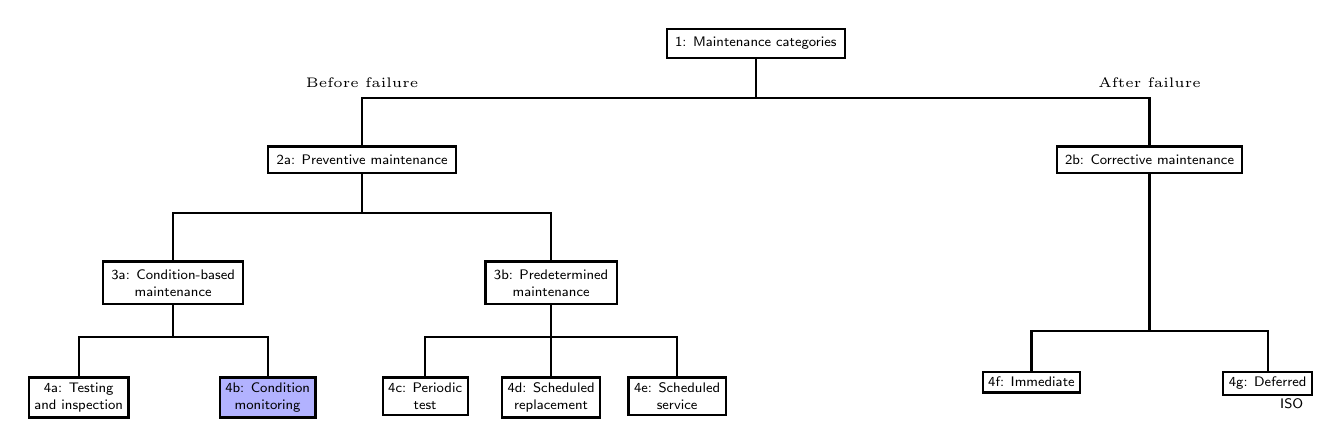
\begin{tikzpicture}[
      font=\sffamily\tiny,
      box/.style={rectangle, draw, thick, align=center, inner sep=3pt},
      smallbox/.style={rectangle, draw, thick, align=center, inner sep=2pt},
    ]

    % --- NIVEL 1 ---
    \node[box] (n1) {1: Maintenance categories};

    % Etiquetas de las ramas principales
    \node[font=\tiny, fill=white, inner sep=1pt] at ($(n1.south) + (-5.0,-0.3)$) {Before failure};
    \node[font=\tiny, fill=white, inner sep=1pt] at ($(n1.south) + (5.0,-0.3)$) {After failure};

    % Conexiones Nivel 1 a Nivel 2
    \draw[thick] (n1.south) -- ++(0,-0.5) -| ($(n1.south) + (-5.0,-1.1)$);
    \draw[thick] (n1.south) -- ++(0,-0.5) -| ($(n1.south) + (5.0,-1.1)$);

    % --- NIVEL 2 ---
    \node[box] (n2a) [below=1.1cm of n1, xshift=-5.0cm] {2a: Preventive maintenance};
    \node[box] (n2b) [below=1.1cm of n1, xshift=5.0cm] {2b: Corrective maintenance};

    % --- NIVEL 3 (Preventivo) ---
    \draw[thick] (n2a.south) -- ++(0,-0.5) -| ($(n2a.south) + (-2.4,-1.1)$);
    \draw[thick] (n2a.south) -- ++(0,-0.5) -| ($(n2a.south) + (2.4,-1.1)$);

    \node[box] (n3a) [below=1.1cm of n2a, xshift=-2.4cm] {3a: Condition-based\\maintenance};
    \node[box] (n3b) [below=1.1cm of n2a, xshift=2.4cm] {3b: Predetermined\\maintenance};

    % --- NIVEL 4 (Bajo 3a) ---
    \draw[thick] (n3a.south) -- ++(0,-0.4) -| ($(n3a.south) + (-1.2,-0.9)$);
    \draw[thick] (n3a.south) -- ++(0,-0.4) -| ($(n3a.south) + (1.2,-0.9)$);

    \node[smallbox] (n4a) [below=0.9cm of n3a, xshift=-1.2cm] {4a: Testing\\and inspection};
    \node[smallbox, fill=blue!30] (n4b) [below=0.9cm of n3a, xshift=1.2cm] {4b: Condition\\monitoring};

    % --- NIVEL 4 (Bajo 3b - Predictivo) ---
    \draw[thick] (n3b.south) -- ++(0,-0.4) -| ($(n3b.south) + (-1.6,-0.9)$);
    \draw[thick] (n3b.south) -- ++(0,-0.4) -| ($(n3b.south) + (0,-0.9)$);
    \draw[thick] (n3b.south) -- ++(0,-0.4) -| ($(n3b.south) + (1.6,-0.9)$);

    \node[smallbox] (n4c) [below=0.9cm of n3b, xshift=-1.6cm] {4c: Periodic\\test};
    \node[smallbox] (n4d) [below=0.9cm of n3b, xshift=0cm] {4d: Scheduled\\replacement};
    \node[smallbox] (n4e) [below=0.9cm of n3b, xshift=1.6cm] {4e: Scheduled\\service};

    % --- NIVEL 4 (Bajo 2b - Correctivo) ---
    \draw[thick] (n2b.south) -- ++(0,-2.0) -| ($(n2b.south) + (-1.5,-2.5)$);
    \draw[thick] (n2b.south) -- ++(0,-2.0) -| ($(n2b.south) + (1.5,-2.5)$);

    \node[smallbox] (n4f) [below=2.5cm of n2b, xshift=-1.5cm] {4f: Immediate};
    \node[smallbox] (n4g) [below=2.5cm of n2b, xshift=1.5cm] {4g: Deferred};

    % --- ETIQUETA IEC ---
    \node[font=\sffamily\tiny, anchor=south east] at (current bounding box.south east) {ISO};

  \end{tikzpicture}

  % Restaura los shorthands de babel
  \shorthandon{>}

  \caption{Diagrama de categorías de mantenimiento.}
  \label{fig:maintenance_categories}
\end{figure}

El \gls{PdM} puede utilizar diferentes métodos, que se pueden clasificar en tres grandes grupos (figura
\ref{fig:predictive_maintenance_methods}). Los \textit{\textbf{métodos basados en modelos de mecanismos}} utilizan
principalmente ecuaciones matemáticas para describir el comportamiento físico de los sistemas y predecir su vida útil.
Los \textit{\textbf{métodos basados en datos}} emplean principalmente técnicas de \gls{ml} para analizar grandes
volúmenes de datos históricos y detectar patrones que indiquen un fallo inminente. Por último, los
\textit{\textbf{métodos híbridos}} combinan ambos enfoques, aprovechando las ventajas de cada uno para mejorar la
precisión de las predicciones.

\begin{figure}[H]
  \centering
  % Desactiva los shorthands activos de babel para evitar conflictos con TikZ
  \shorthandoff{>}

  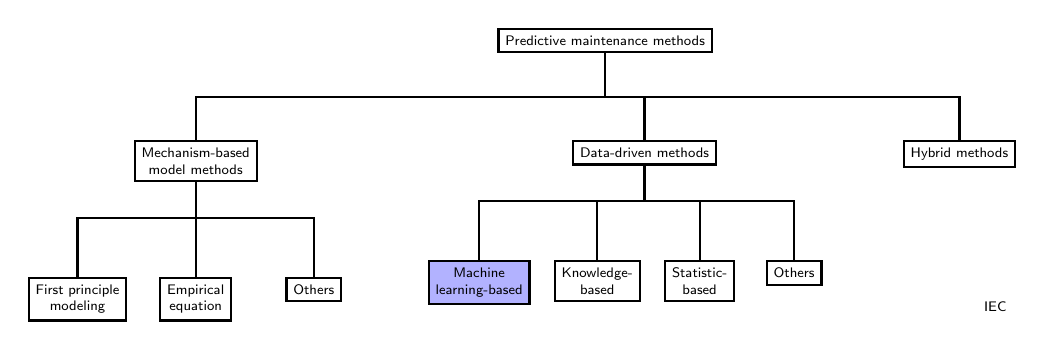
\begin{tikzpicture}[
      font=\sffamily\tiny, % Tamaño tiny para todo el diagrama
      box/.style={
          rectangle,
          draw=black,
          thick,
          align=center,
          inner sep=2.5pt,
          fill=white
        }
    ]

    % --- NIVEL 1 (Raíz) ---
    \node[box] (root) {Predictive maintenance methods};

    % --- NIVEL 2 ---
    \node[box] (n2a) [below=1.1cm of root, xshift=-5.2cm] {Mechanism-based\\model methods};
    \node[box] (n2b) [below=1.1cm of root, xshift=0.5cm]   {Data-driven methods};
    \node[box] (n2c) [below=1.1cm of root, xshift=4.5cm]  {Hybrid methods};

    % Conexiones Nivel 1 a Nivel 2
    \draw[thick] (root.south) -- ++(0,-0.55) -| (n2a.north);
    \draw[thick] (root.south) -- ++(0,-0.55) -| (n2b.north);
    \draw[thick] (root.south) -- ++(0,-0.55) -| (n2c.north);

    % --- NIVEL 3 (Subniveles de n2a) ---
    \node[box] (n3a) [below=1.2cm of n2a, xshift=-1.5cm] {First principle\\modeling};
    \node[box] (n3b) [below=1.2cm of n2a, xshift=0cm]    {Empirical\\equation};
    \node[box] (n3c) [below=1.2cm of n2a, xshift=1.5cm]  {Others};

    % La bajada (-0.45) es idéntica en n2a y n2b para alinear las líneas horizontales
    \draw[thick] (n2a.south) -- ++(0,-0.45) -| (n3a.north);
    \draw[thick] (n2a.south) -- ++(0,-0.45) -| (n3b.north);
    \draw[thick] (n2a.south) -- ++(0,-0.45) -| (n3c.north);

    % --- NIVEL 3 (Subniveles de n2b ---
    \node[box, fill=blue!30] (n3d) [below=1.2cm of n2b, xshift=-2.1cm] {Machine\\learning-based};
    \node[box] (n3e) [below=1.2cm of n2b, xshift=-0.6cm] {Knowledge-\\based};
    \node[box] (n3f) [below=1.2cm of n2b, xshift=0.7cm]  {Statistic-\\based};
    \node[box] (n3g) [below=1.2cm of n2b, xshift=1.9cm]  {Others};

    \draw[thick] (n2b.south) -- ++(0,-0.45) -| (n3d.north);
    \draw[thick] (n2b.south) -- ++(0,-0.45) -| (n3e.north);
    \draw[thick] (n2b.south) -- ++(0,-0.45) -| (n3f.north);
    \draw[thick] (n2b.south) -- ++(0,-0.45) -| (n3g.north);

    % --- ETIQUETA IEC ---
    \node[font=\sffamily\tiny, anchor=south east] at (current bounding box.south east) {IEC};

  \end{tikzpicture}

  % Restaura los shorthands de babel
  \shorthandon{>}

  \caption{Diagrama jerárquico de métodos de mantenimiento predictivo.}
  \label{fig:predictive_maintenance_methods}
\end{figure}

La elección de la estrategia analítica depende directamente de los datos disponibles (historial de fallos, registros de
sensores, datos operativos) y del objetivo operativo. A continuación se detallan las cuatro estrategias principales,
analizando sus ventajas y limitaciones. Las estrategias marcadas con un asterisco no se abordan en este trabajo.

\begin{itemize}
  \item \textbf{Regresión (RUL)}: Modelos de regresión para predecir la \gls{RUL}
        \begin{itemize}
          \item \textbf{Ventaja}: Permite estimar el tiempo exacto hasta el fallo, facilitando la planificación de
                intervenciones de mantenimiento y la optimización de recursos.
          \item \textbf{Limitación}: Requiere datos históricos completos que incluyan el ciclo completo de vida del
                equipo, desde su inicio hasta su fallo, lo cual puede ser difícil de obtener en entornos industriales.
        \end{itemize}
  \item \textbf{Clasificación}: Modelos de clasificación para predecir la probabilidad de fallo en una ventana temporal
        \begin{itemize}
          \item \textbf{Ventaja}: Proporciona una alerta temprana sobre la probabilidad de fallo en un período
                específico, lo que permite tomar decisiones operativas inmediatas.
          \item \textbf{Limitación}: La definición de la ventana temporal puede ser subjetiva y afectar la precisión del
                modelo; además, requiere datos históricos con marcas de pre-fallo.
        \end{itemize}
  \item \textbf{Detección de anomalías}\textsuperscript{*}: Modelos de detección de anomalías para identificar patrones
        inusuales en los datos de sensores que puedan indicar un fallo inminente
        \begin{itemize}
          \item \textbf{Ventaja}: No requiere datos de fallos previos, lo que permite detectar problemas emergentes en
                equipos nuevos o poco documentados.
          \item \textbf{Limitación}: No proporciona información sobre el tiempo exacto hasta el fallo ni sobre el tipo
                de fallo, lo que puede limitar la capacidad de planificación de mantenimiento.
        \end{itemize}
  \item \textbf{Análisis de supervivencia}\textsuperscript{*}: Modelos de análisis de supervivencia para estimar la
        probabilidad de fallo a lo largo del tiempo, considerando censura y eventos de interés
        \begin{itemize}
          \item \textbf{Ventaja}: Permite gestionar equipos que aún no han fallado, proporcionando información sobre la
                probabilidad de fallo en función del tiempo y facilitando la planificación de mantenimiento preventivo.
          \item \textbf{Limitación}: Requiere un modelado matemático más complejo y puede ser sensible a la calidad y
                cantidad de datos censurados disponibles.
        \end{itemize}
\end{itemize}

\begingroup
\footnotesize
\setlength{\LTcapwidth}{\textwidth}
\begin{longtable}{| >{\raggedright\arraybackslash}p{2.5cm} | >{\raggedright\arraybackslash}p{2.8cm} | >{\raggedright\arraybackslash}p{3.0cm} | >{\raggedright\arraybackslash}p{3.2cm} | >{\raggedright\arraybackslash}p{2.5cm} |}
  \caption{\mbox{Tabla comparativa de estrategias para Mantenimiento Predictivo}}
  \label{tab:estrategias_mantenimiento_predictivo}                                                                                                                                                                                            \\

  % --- CABECERA PARA LA PRIMERA PÁGINA ---
  \hline
  \textbf{Estrategia}          & \textbf{Tipo de Objetivo}                         & \textbf{Datos Históricos Necesarios}             & \textbf{Ventaja Principal}                          & \textbf{Principal Limitación}                   \\
  \hline
  \endfirsthead

  % --- CABECERA PARA LAS SIGUIENTES PÁGINAS ---
  \multicolumn{5}{c}{{\tablename} \thetable{} -- Continuación de la página anterior}                                                                                                                                                          \\[0.5em]
  \hline
  \textbf{Estrategia}          & \textbf{Tipo de Objetivo}                         & \textbf{Datos Históricos Necesarios}             & \textbf{Ventaja Principal}                          & \textbf{Principal Limitación}                   \\
  \hline
  \endhead

  % --- PIE DE PÁGINA PARA CUANDO LA TABLA CONTINÚA ---
  \hline
  \multicolumn{5}{r}{\textit{Continúa en la página siguiente...}}                                                                                                                                                                             \\
  \endfoot

  % --- PIE DE PÁGINA PARA LA ÚLTIMA PÁGINA ---
  \hline
  \endlastfoot

  % --- CONTENIDO DE LA TABLA ---
  1. Regresión (RUL)           & Continuo (Tiempo exacto hasta fallo)              & Completos (De inicio a rotura)                   & Máxima precisión en la planificación                & Muy difícil conseguir datos de roturas reales   \\
  \hline
  2. Clasificación (Ventana)   & Binario / Categórico ($\sim$¿Falla en $X$ horas?) & Historiales con marcas de pre-fallo              & Práctico para la operación real y logística         & Sensible a la definición de la ventana temporal \\
  \hline
  \rowcolor{gray!30}
  3. Detección de Anomalías    & No supervisado (Normal vs. Anómalo)               & Solo datos de funcionamiento normal              & No requiere datos de fallos previos                 & No predice el tiempo ni el tipo de fallo        \\
  \hline
  \rowcolor{gray!30}
  4. Análisis de Supervivencia & Probabilidad de fallo en función del tiempo       & Historiales con datos censurados (activos vivos) & Excelente gestión de equipos que aún no han fallado & Modelado matemático más complejo                \\
  \hline
\end{longtable}
\footnotesize \textit{Nota:} Las filas de color gris indican las estrategias que no se implementan en este trabajo.
\endgroup

\section{Estado del Arte}

\subsection{Descripción de publicaciones relacionadas con la temática}

A continuación, se presentan artículos que emplean modelos de clasificación para estimar la probabilidad de fallo
dentro de una ventana temporal:

\begin{itemize}
  \item Improving rail network velocity: A machine learning approach to predictive maintenance \cite{li2014improving}
        \begin{itemize}
          \item \textbf{Enfoque de clasificación}: Se desarrolla un modelo de clasificación personalizado basado en
                \gls{svm} para predecir alarmas asociadas a fallos catastróficos, como el sobrecalentamiento de
                rodamientos, a partir de la combinación de datos procedentes de varios detectores instalados en las vías.
          \item \textbf{Ventana temporal y alerta temprana}: Se generan predicciones con una antelación de 3 y 7 días,
                lo que proporciona un margen suficiente para realizar inspecciones proactivas y prevenir paradas de
                trenes e interrupciones del servicio. Asimismo, se emplean árboles de decisión para clasificar y
                predecir defectos en los bastidores y las ruedas de los vagones con una antelación de hasta 3 meses.
        \end{itemize}
  \item Análisis estadístico de datos para el mantenimiento predictivo de maquinaria industrial \cite{brasa2019analisis}
        \begin{itemize}
          \item \textbf{Enfoque de clasificación}: Se implementa explícitamente un modelo de clasificación orientado al
                mantenimiento predictivo mediante ensembles de árboles de decisión, como \gls{RandomForest} y \gls{XGBoost}.
          \item \textbf{Ventana temporal y alerta temprana}: La variable objetivo se diseña para estimar la probabilidad
                de que la máquina sufra una avería durante los próximos $A$ ciclos, con un intervalo definido en el
                estudio de entre 10 y 100 ciclos. Se genera una alerta temprana, mediante la asignación de la clase 1,
                cuando se prevé una parada imprevista dentro de dicho periodo, lo que facilita la toma de decisiones
                operativas.
        \end{itemize}
  \item Predictive Maintenance using \gls{lstm} and Adaptive Windowing \cite{adivi2024predictive}
        \begin{itemize}
          \item \textbf{Enfoque de clasificación}: El enfoque de clasificación se basa en una arquitectura de redes
                \gls{lstm} estructurada en múltiples ramas independientes, donde cada una se encarga de predecir de
                forma específica la probabilidad de fallo para un componente determinado de la máquina. Para resolver
                esta tarea de naturaleza binaria, cada rama incorpora una función de activación sigmoide en su capa de
                salida y emplea la entropía cruzada binaria como función de pérdida para evaluar la discrepancia con las
                etiquetas reales.
          \item \textbf{Ventana temporal y alerta temprana}: El modelo prescinde de los tamaños fijos convencionales e
                implementa una estrategia adaptativa basada en optimización bayesiana para ajustar dinámicamente el
                tamaño de la ventana de entrada. Mediante el uso de técnicas de ventana deslizante superpuesta, el
                sistema equilibra el contexto histórico necesario para capturar las dinámicas de degradación y maximiza
                la precisión de las predicciones anticipadas para evitar fallos operativos inesperados
        \end{itemize}
  \item A Transformer Approach for Remaining Useful Life Prediction and Fault Diagnosis of Mechanical Equipment
        \cite{liu2026transformer}
        \begin{itemize}
          \item \textbf{Enfoque}: El estudio propone un marco basado en una arquitectura \gls{transformer} compartida
                para realizar simultáneamente la predicción de la vida útil restante y la clasificación multietiqueta de
                fallos en equipos mecánicos a través de la captura de dependencias temporales y cruzadas entre sensores.
          \item \textbf{Optimización}: La optimización central se basa en una estrategia de ponderación de pérdidas
                guiada por la incertidumbre que equilibra de manera automática el entrenamiento de ambas tareas,
                estabilizando la convergencia y permitiendo alcanzar un rendimiento superior en comparación con los
                modelos de referencia tradicionales y de aprendizaje profundo.
        \end{itemize}
\end{itemize}

A continuación, se presentan artículos que emplean modelos de regresión para predecir la \gls{RUL} (\gls{rul}):

\begin{itemize}
  \item Análisis estadístico de datos para el mantenimiento predictivo de maquinaria industrial \cite{brasa2019analisis}
        \begin{itemize}
          \item \textbf{Enfoque}: Este trabajo se centra en la predicción de \gls{rul} utilizando un modelo de regresión
                de dos capas (una primera capa con \gls{RandomForest} para reducir dimensionalidad y extraer curvas de
                degradación, y una segunda capa con \gls{XGBoost}).
          \item \textbf{Optimización}: Se implementan y comparan funciones de penalización personalizadas (cuadráticas e
                inversas) en la función objetivo y de evaluación de \gls{XGBoost} para minimizar el \gls{rmse} evitando
                predecir valores de RUL superiores a los reales, lo cual es crítico para evitar paradas imprevistas y
                optimizar la planificación de intervenciones.
        \end{itemize}
  \item Forecasting Fault Events for Predictive Maintenance using Data-driven Techniques and ARMA Modeling
        \cite{baptista2017forecasting}
        \begin{itemize}
          \item \textbf{Enfoque}: Se propone un marco analítico combinado que integra modelos de series temporales
                (\gls{arma}) con técnicas de regresión impulsadas por datos (\gls{svr}, regresión lineal generalizada,
                \gls{RandomForest}, k-NN y \gls{RedesNeuronales}).
          \item \textbf{Utilidad}: Su objetivo es predecir en línea el momento exacto del próximo evento de fallo o
                retirada de un componente crítico (válvulas de motores de aviones), superando a los modelos
                tradicionales de Weibull y reduciendo tanto las intervenciones innecesarias como los fallos no
                planificados.
        \end{itemize}
  \item A Transformer Approach for Remaining Useful Life Prediction and Fault Diagnosis of Mechanical Equipment
        \cite{liu2026transformer}
        \begin{itemize}
          \item \textbf{Enfoque}: El estudio propone un marco basado en una arquitectura \gls{transformer} compartida
                para realizar simultáneamente la predicción de la vida útil restante y la clasificación multietiqueta de
                fallos en equipos mecánicos a través de la captura de dependencias temporales y cruzadas entre sensores.
          \item \textbf{Optimización}: La optimización central se basa en una estrategia de ponderación de pérdidas
                guiada por la incertidumbre que equilibra de manera automática el entrenamiento de ambas tareas,
                estabilizando la convergencia y permitiendo alcanzar un rendimiento superior en comparación con los
                modelos de referencia tradicionales y de aprendizaje profundo.
        \end{itemize}
\end{itemize}

En el ámbito del mantenimiento predictivo industrial, la evolución de las técnicas analíticas ha partido de modelos
estadísticos de series temporales, como \gls{arima} \cite{kanawaday2017machine}, concebidos para pronosticar el
comportamiento de la maquinaria, facilitar la planificación de las intervenciones y adaptar la producción.
Históricamente, estos enfoques se han complementado con algoritmos de clasificación clásicos, como \gls{svm}, que,
junto con técnicas de ingeniería de características, reducen la dimensionalidad de los datos. Esta simplicidad
algorítmica resulta especialmente idónea para entornos de \gls{edgecomputing} con recursos limitados donde se requiere
un procesamiento ágil en tiempo real \cite{mian2023artificial}.

Con el incremento en la recopilación de datos asociado a la \gls{i40}, el análisis predictivo ha transitado hacia
arquitecturas de aprendizaje profundo más complejas, aunque su aplicación en entornos reales exige superar importantes
barreras de preprocesamiento. A menudo, resulta necesario segmentar las señales en bruto para aislar operaciones
específicas de cada herramienta. Para ello, se emplean flujos de trabajo que integran agrupamiento no supervisado, como
k-means \cite{kounta2023deep}, con el fin de etiquetar fases de producción automáticamente. Estas estrategias se
combinan con clasificadores basados en \gls{dt} y \gls{RedesNeuronalesConvolucionales} \cite{zufle2022machine}. En esta
misma línea, la transformación de señales unidimensionales de vibración en imágenes bidimensionales en el dominio de la
frecuencia ha permitido abordar el diagnóstico de fallos como un problema de visión por computador, facilitando la
monitorización inteligente e identificación autónoma de anomalías \cite{kounta2023deep}.

A pesar de estos avances, los modelos suelen enfrentarse al desafío del desequilibrio entre clases, dado que las averías
son eventos poco frecuentes. Para mitigar la falta de datos representativos de la clase minoritaria, se recurre a la
generación de datos sintéticos mediante redes como StyleGAN \cite{kim2023self}, lo que favorece el entrenamiento de
clasificadores más equilibrados. Como alternativa orientada a la detección no supervisada, se usan de arquitecturas
robustas frente al ruido, como los autoencoders convolucionales híbridos (HRCAE) \cite{yan2023hybrid}, que detectan
anomalías de forma fiable sin depender de grandes volúmenes de datos previamente etiquetados.

La necesidad de modelar secuencias temporales cada vez más complejas y capturar dependencias a largo plazo ha impulsado
la transición del mantenimiento predictivo hacia el paradigma introducido por el artículo \textit{Attention Is All You Need}\cite{vaswani2017attention_neurips}.
La integración de mecanismos de atención a través de arquitecturas \gls{transformer} ha supuesto un salto cualitativo
respecto a las redes recurrentes y convolucionales, al permitir que el modelo pondere dinámicamente la relevancia de los
diferentes instantes temporales en las señales sensoriales, extrayendo patrones de degradación sutiles con una alta
precisión.

Enmarcado en esta evolución metodológica, el presente trabajo analiza un flujo reproducible basado en el conjunto de
datos Microsoft Azure Predictive Maintenance \cite{biswas_microsoft_azure_predictive_maintenance}. Se lleva a cabo la
preparación temporal de los datos, la ingeniería de características y la comparación de diversos algoritmos orientados a
dos objetivos complementarios: la detección de fallos en una ventana de tiempo y la estimación de la vida útil restante
(\gls{rul}). Como aportación principal, se propone optimizar una arquitectura \gls{transformer} multitarea \cite{liu2026transformer}
sustituyendo su capa de calibración lineal por un cabezal fundamentado en el análisis de supervivencia. De este modo, en
lugar de predecir un único valor continuo para la \gls{rul}, el cabezal genera los parámetros de una distribución de
probabilidad temporal, como la \gls{weibull} \cite{maragallcambra2018}, o bien probabilidades de riesgo discretas para
diferentes intervalos. Esta adaptación no solo incrementa la robustez estadística de las estimaciones, sino que mejora
notablemente la interpretabilidad de la red Transformer en el diagnóstico industrial.

\subsection{Tabla Resumen}

En la tabla \ref{tab:resumen_literatura} se presenta un resumen de los trabajos revisados, incluyendo información sobre
los autores, el sector industrial, las variables utilizadas, los algoritmos o técnicas de \gls{ml} aplicadas y las
métricas de evaluación empleadas para medir el rendimiento de los modelos predictivos. Esta tabla proporciona una visión
general de la diversidad de enfoques y metodologías utilizadas en el ámbito del \gls{PdM} industrial, destacando las
tendencias y las mejores prácticas identificadas en la revisión bibliográfica.

\begingroup
\scriptsize
\setlength{\LTcapwidth}{\textwidth}
\begin{longtable}{| >{\raggedright\arraybackslash}p{1.9cm} | >{\raggedright\arraybackslash}p{1.8cm} | >{\raggedright\arraybackslash}p{2.8cm} | >{\raggedright\arraybackslash}p{2.8cm} | >{\raggedright\arraybackslash}p{2.1cm} | >{\centering\arraybackslash}p{2.1cm} |}  \caption{Tabla resumen de la bibliografía revisada}
  \label{tab:resumen_literatura}                                                                                                                                                                                                                                                                                                                                                                                                                                                                        \\

  % --- CABECERA PARA LA PRIMERA PÁGINA ---
  \hline
  \textbf{Autor / Año}                                             & \textbf{Sector Industrial}                             & \textbf{Variables Utilizadas}                                                                          & \textbf{Algoritmos / Técnicas de ML}                                                                                      & \textbf{Métricas de evaluación}                                                                              & \textbf{Presente TFM} \\
  \hline
  \endfirsthead

  % --- CABECERA PARA LAS SIGUIENTES PÁGINAS ---
  \multicolumn{5}{c}{{\tablename} \thetable{} -- Continuación de la página anterior}                                                                                                                                                                                                                                                                                                                                                                                                                    \\[0.5em]
  \hline
  \textbf{Autor / Año}                                             & \textbf{Sector Industrial}                             & \textbf{Variables Utilizadas}                                                                          & \textbf{Algoritmos / Técnicas de ML}                                                                                      & \textbf{Métricas de evaluación}                                                                              & \textbf{Presente TFM} \\
  \hline
  \endhead

  % --- PIE DE PÁGINA PARA CUANDO LA TABLA CONTINÚA ---
  \hline
  \multicolumn{5}{r}{\textit{Continúa en la página siguiente...}}                                                                                                                                                                                                                                                                                                                                                                                                                                       \\
  \endfoot

  % --- PIE DE PÁGINA PARA LA ÚLTIMA PÁGINA ---
  \hline
  \endlastfoot

  % --- CONTENIDO DE LA TABLA ---
  Li et al., 2014 \cite{li2014improving}                           & Ferroviario (US Class I railroad)                      & Datos de detectores en vía (HBD, WILD, ABD, OGD, TPD), fallas históricas, mantenimiento y clima        & Análisis de correlación, análisis causal, series temporales, \gls{svm} personalizado, Árboles de Decisión                 & \gls{tpr}, \gls{fpr}                                                                                         &                       \\
  \hline
  Baptista et al., 2017 \cite{baptista2017forecasting}             & Aeronáutica / Aviación                                 & Datos temporales de historial de uso y retiradas (sin sensores)                                        & \gls{arma}, \gls{svr}, \gls{glm}, KNN, \gls{RandomForest}, \gls{RedesNeuronales}                                          & \gls{rmse}, \gls{mape}, \gls{mae}, \gls{mdae}, MTBF                                                          &                       \\
  \hline
  \rowcolor{gray!30}
  Kanawaday \& Sane, 2017 \cite{kanawaday2017machine}              & Manufactura / Empaquetado                              & Sensores \gls{iot}: Tensión, Presión, Ancho, Diámetro                                                  & \gls{arima}, Naive Bayes, \gls{svm}, CART, \gls{dnn}                                                                      & \gls{precisión}                                                                                              &                       \\
  \hline
  Maragall Cambra, 2018                                            & Aeronáutica / Aviación                                 & Datos temporales de historial de uso y retiradas (sin sensores)                                        & Weibull Time To Event (WTTE-RNN)                                                                                          & \gls{mae}, \gls{rmse}, $R^2$                                                                                 & X                     \\
  \hline
  Brasa Estévez, 2019 \cite{brasa2019analisis}                     & Aeroespacial (Simulación NASA)                         & Datos de 27 sensores de monitorización a lo largo de ciclos                                            & Ensembles: Bagging (\gls{RandomForest}), Boosting (\gls{XGBoost})                                                         & \gls{rmse}, \gls{auc}, N (predicciones excedidas)                                                            &                       \\
  \hline
  \rowcolor{gray!30}
  Justus \& Kanagachidambaresan, 2022 \cite{justus2022intelligent} & Máquinas CNC / Manufactura                             & Vibración (\gls{fft}), Temperatura, Humedad, Humo, Diámetro manual                                     & Regresión Lineal, KNN, \gls{RandomForest}, \gls{svm}                                                                      & \gls{precisión}                                                                                              &                       \\
  \hline
  \rowcolor{gray!30}
  Lizcano, C., 2022 \cite{lizcano2022mantenimiento}                & Centro de datos                                        & Voltaje, rotación, presión, vibración, indicadores de error, indicadores de mantenimiento y antigüedad & \gls{RandomForest}, \gls{XGBoost}                                                                                         & \gls{precisión}, \gls{exhaustividad}, F1-Score, \gls{rmse}                                                   &                       \\
  \hline
  \rowcolor{gray!30}
  Züfle et al., 2022 \cite{zufle2022machine}                       & Máquinas herramientas CNC                              & Datos internos (posición, velocidad, torque, potencia, temp) y vibración 3-ejes                        & Clustering jerárquico, \gls{RandomForest}, Decision Tree, \gls{XGBoost}, \gls{svm}, KNN, Regresión Logística, Naive Bayes & \gls{precisión}, \gls{exactitud}, \gls{exhaustividad}, F1-Score, \gls{mcc}                                   &                       \\
  \hline
  \rowcolor{gray!30}
  Kim et al., 2023 \cite{kim2023self}                              & Máquinas CNC y Soldadura WAAM                          & Fuerza (x,y,z), Vibración (x,y,z), Emisión Acústica, Corriente, Voltaje (convertidos a imágenes GAF)   & StyleGAN (aumento de datos), \gls{XGBoost}, AdaBoost, Gradient Boost                                                      & \gls{precisión}, \gls{exactitud}, \gls{exhaustividad}, F1-Score                                              &                       \\
  \hline
  \rowcolor{gray!30}
  Kounta et al., 2023 \cite{kounta2023deep}                        & Metalmecánico (Ferroviario TGV)                        & Señales de vibración transformadas mediante \gls{fft} a imágenes                                       & Transfer Learning (\gls{dl}): VGG16, ResNet50                                                                             & \gls{precisión}, \gls{exactitud}, \gls{exhaustividad}, F1-Score                                              &                       \\
  \hline
  \rowcolor{gray!30}
  Mian et al., 2023 \cite{mian2023artificial}                      & Maquinaria rotativa (Motores, engranajes, rodamientos) & Vibración (acelerómetro MPU6050, 9 características estadísticas)                                       & Naive Bayes, k-NN, RNN, \gls{svm} (\gls{aiot} / \gls{edgecomputing})                                                      & \gls{precisión}, \gls{exactitud}, \gls{exhaustividad}, \gls{especificidad}, F1-Score, \gls{mcc}, \gls{kappa} &                       \\
  \hline
  \rowcolor{gray!30}
  Yan et al., 2023 \cite{yan2023hybrid}                            & Máquinas herramientas CNC                              & Señales de vibración multicanal en 3 ejes (X, Y, Z) en el dominio de la frecuencia (con ruido añadido) & HRCAE (Hybrid Robust Convolutional Autoencoder), módulo PCDF, función de pérdida FDD                                      & \gls{precisión}, \gls{exactitud}, \gls{exhaustividad}, F-score, \gls{auc}                                    &                       \\
  \hline
  Adivi et al., 2024 \cite{adivi2024predictive}                    & Centro de datos                                        & Voltaje, rotación, presión, vibración, indicadores de error, indicadores de mantenimiento y antigüedad & Redes \gls{lstm} con ventana deslizante adaptativa y optimización bayesiana                                               & \gls{precisión}                                                                                              &                       \\
  \hline
  Yuchen et al., 2026 \cite{liu2026transformer}                    & Centro de datos                                        & Voltaje, rotación, presión, vibración, indicadores de error, indicadores de mantenimiento y antigüedad & Arquitectura \gls{transformer} multitarea con codificador compartido y cabezas duales                                     & \gls{mae}, \gls{rmse}, F1-score, \gls{precisión}                                                             & X                     \\
  \hline
\end{longtable}
\footnotesize \textit{Nota:} Las filas de color gris se centran en la detección de fallos, que puede utilizarse para
etiquetar automáticamente los datos antes de la fase de modelado.
\endgroup

\subsection{Conclusiones del Estado del Arte}

La revisión muestra que el mantenimiento predictivo no es una tarea única, sino un conjunto de problemas relacionados:
detección de anomalías, clasificación de estados de funcionamiento, predicción de fallos y estimación de la vida útil
restante (\gls{rul}). Los datos de sensores \gls{iot} permiten capturar cambios graduales en el comportamiento de los
equipos, pero su utilidad depende de cómo se definan las variables, las ventanas temporales y las etiquetas. En este
sentido, los trabajos revisados sobre el conjunto de datos Microsoft Azure Predictive Maintenance
\cite{biswas_microsoft_azure_predictive_maintenance} ilustran tanto el interés práctico del conjunto como la diversidad
de objetivos que pueden construirse a partir de él \cite{lizcano2022mantenimiento,d4rklucif3r_predictive_maintenance}.
Las propuestas más recientes amplían las posibilidades del modelado, por ejemplo mediante ventanas adaptativas en redes
\gls{lstm} \cite{adivi2024predictive} o mediante arquitecturas \gls{transformer} para combinar la predicción de
\gls{rul} y el diagnóstico de fallos \cite{liu2026transformer}; sin embargo, una arquitectura más compleja no garantiza
por sí misma una mejor decisión de mantenimiento.

La evidencia comparada no permite identificar un algoritmo universalmente superior. El rendimiento depende del tipo de
fallo, la frecuencia de muestreo, la calidad de las etiquetas, el horizonte de predicción, el ruido y la distribución de
los datos. Los modelos estadísticos y los clasificadores clásicos pueden ofrecer soluciones interpretables y de coste
reducido, mientras que los métodos de aprendizaje profundo pueden aprovechar dependencias temporales o representaciones
complejas; la elección debe responder a las características del problema y a las restricciones operativas, no a la
sofisticación del algoritmo. Además, los fallos son acontecimientos minoritarios: un modelo puede alcanzar una exactitud
elevada ignorando precisamente la clase que se pretende anticipar. El desequilibrio exige estrategias específicas de
preparación y evaluación, como el aumento controlado de la clase minoritaria \cite{kim2023self}, y obliga a analizar
conjuntamente la \gls{precisión}, la \gls{exhaustividad}, F1, la \gls{auc} y la tasa de falsas alarmas. Estas últimas
son especialmente relevantes, porque un exceso de avisos innecesarios puede provocar intervenciones costosas y reducir
la confianza en el sistema \cite{li2014improving}.

Una limitación transversal de los trabajos revisados es la dificultad para comparar sus resultados. Cambian
simultáneamente los equipos, los sensores, la definición de fallo, la ventana de predicción, la partición de los datos y
las métricas; además, algunos estudios emplean datos simulados o experimentales con una representatividad industrial
limitada. Por ello, los resultados publicados no permiten establecer de forma aislada qué modelo es más adecuado para el
conjunto de datos utilizado en este TFM. La literatura tampoco resuelve suficientemente cómo equilibrar, en un mismo
estudio reproducible, la anticipación de la alerta, la detección de fallos minoritarios y el coste de las falsas alarmas
cuando se comparan modelos de distinta complejidad.

\chapter{Diseño e implementación del trabajo}

El entorno de desarrollo del proyecto se fundamenta en el uso de herramientas y bibliotecas de código abierto
ampliamente extendidas en las comunidades científica y de ingeniería de datos. Esta selección permite garantizar la
reproducibilidad de los experimentos, facilitar la colaboración técnica y asegurar una integración fluida con entornos
productivos.

Los cuadernos de Jupyter ofrecen un entorno interactivo en el que se integran código ejecutable, visualizaciones y
documentación dentro de un formato accesible y de sencilla difusión. Su empleo agiliza el análisis exploratorio de
datos, la experimentación con modelos y la exposición ordenada de los resultados obtenidos.

Asimismo, la extensión \texttt{pycodestyle\_magic} permite comprobar directamente en las celdas de Jupyter el ajuste del
código a las convenciones de estilo PEP~8. De este modo, se promueve un código legible, mantenible y alineado con las
buenas prácticas de programación en Python.

\section{Origen de los datos}

En este trabajo se utiliza la versión reducida del conjunto de datos de análisis de mantenimiento predictivo que forma
parte de \href{https://github.com/Azure-Samples/MachineLearningSamples-PredictiveMaintenance}{Advanced Scenario: General Predictive Maintenance}
de la guía de modelado de mantenimiento predictivo para \href{https://github.com/microsoft/SQL-Server-R-Services-Samples}{SQL Server R Services Samples}.

En 2016 Microsoft publica una guía de modelado de mantenimiento predictivo con el objetivo de proporcionar un escenario
práctico para la implementación de soluciones de mantenimiento predictivo en entornos industriales.

El ejemplo de mantenimiento predictivo está disponible hasta el 17 de junio de 2019, momento en el que se archiva el
proyecto y se deja de mantener. La versión reducida se encuentra disponible desde el año 2020 en el repositorio
\href{https://www.kaggle.com/datasets/arnabbiswas1/microsoft-azure-predictive-maintenance/}{Microsoft Azure Predictive Maintenance}.

La versión completa del conjunto de datos, incluye información de 1.000 máquinas industriales, mientras que la versión
reducida contiene datos de 100 máquinas.

El conjunto de datos sintético contiene información de sensores de vibración, temperatura, presión y otros parámetros de
funcionamiento de un conjunto de máquinas industriales. Los datos se recopilan a lo largo del tiempo y se organizan en
registros que incluyen marcas de tiempo, identificadores de máquina, y valores de los sensores. En el esquema de la
figura \ref{fig:machine} se muestran los componentes y que sensores de una máquina industrial que después se reflejan en
los datos capturados.

\begin{figure}[H]
  \centering
  \includegraphics[width=15truecm]{machine.png}
  \caption{Esquema de una máquina y sus sensores.}
  \label{fig:machine}
\end{figure}

\subsection{Obtención de los datos}

Para descargar el conjunto de datos de Kaggle, se emplea la biblioteca \texttt{kagglehub}, que facilita la obtención
directa de conjuntos de datos desde un cuaderno de Jupyter. En concreto, se invoca la función \texttt{dataset\_download}
indicando el identificador del conjunto de datos (``arnabbiswas1/microsoft-azure-predictive-maintenance''); esta
función descarga los archivos correspondientes en la caché local del sistema, gestiona las versiones disponibles y
devuelve la ruta del directorio donde quedan almacenados para su posterior acceso desde el código.

\subsection{Descripción de los datos}

El conjunto de datos está estructurado en cinco archivos CSV, cada uno contiene información específica sobre el uso, el
desgaste y el mantenimiento de las máquinas. El archivo \textit{PdM\_telemetry.csv} contiene los datos recogidos de los
sensores de las máquinas, incluyendo valores de vibración, temperatura, presión y otros parámetros de funcionamiento.
El archivo \textit{PdM\_errors.csv} contiene información sobre los errores de las máquinas, incluyendo el tipo de error y
la fecha en que ocurrió. El archivo \textit{PdM\_maint.csv} contiene información sobre los eventos de mantenimiento
realizados en las máquinas, incluyendo la fecha y el tipo de mantenimiento. El archivo \textit{PdM\_failures.csv}
contiene información sobre los fallos de las máquinas, incluyendo la fecha y el tipo de fallo. Finalmente, el archivo
\textit{PdM\_machines.csv} contiene información sobre las máquinas, incluyendo su identificador, el tipo de máquina y su
antigüedad.

\begin{figure}[H]
  \centering
  \includegraphics[width=14truecm]{ER.png}
  \caption{Diagrama de entidades y relaciones.}
  \label{fig:er}
\end{figure}

\subsubsection{PdM\_telemetry.csv (Datos de telemetría)}

Es el archivo más grande del conjunto y contiene las lecturas continuas de los sensores de las máquinas registradas con
una frecuencia de 1 hora.

\begingroup
\setlength{\LTcapwidth}{\textwidth}
\begin{longtable}{| >{\ttfamily\raggedright\arraybackslash}p{3.2cm} | >{\raggedright\arraybackslash}p{6.5cm} | >{\raggedright\arraybackslash}p{4.2cm} |}
  \caption{Variables del archivo \texttt{PdM\_telemetry.csv}}
  \label{tab:telemetry_variables}                                                                 \\

  % --- CABECERA PARA LA PRIMERA PÁGINA ---
  \hline
  \normalfont\textbf{Variable} & \textbf{Descripción}                     & \textbf{Tipo}         \\
  \hline
  \endfirsthead

  % --- CABECERA PARA LAS SIGUIENTES PÁGINAS ---
  \multicolumn{3}{c}{{\tablename} \thetable{} -- Continuación de la página anterior}              \\[0.5em]
  \hline
  \normalfont\textbf{Variable} & \textbf{Descripción}                     & \textbf{Tipo}         \\
  \hline
  \endhead

  % --- PIE DE PÁGINA PARA CUANDO LA TABLA CONTINÚA ---
  \hline
  \multicolumn{3}{r}{\textit{Continúa en la página siguiente...}}                                 \\
  \endfoot

  % --- PIE DE PÁGINA PARA LA ÚLTIMA PÁGINA ---
  \hline
  \endlastfoot

  % --- CONTENIDO DE LA TABLA ---
  \texttt{datetime}            & Marca de tiempo de la lectura del sensor & Temporal              \\
  \hline
  \texttt{machineID}           & Identificador único de la máquina        & Categórica nominal    \\
  \hline
  \texttt{volt}                & Voltaje de la máquina                    & Cuantitativa continua \\
  \hline
  \texttt{rotate}              & Velocidad de rotación de la máquina      & Cuantitativa continua \\
  \hline
  \texttt{pressure}            & Presión de la máquina                    & Cuantitativa continua \\
  \hline
  \texttt{vibration}           & Vibración de la máquina                  & Cuantitativa continua \\
  \hline
\end{longtable}
\endgroup

\subsubsection{PdM\_errors.csv (Registro de errores)}

Registro de alertas o códigos de error no críticos que lanzan las máquinas durante su operación. Un error no detiene
la máquina ni significa necesariamente una avería inmediata, pero suele ser un síntoma previo a un fallo.

\begingroup
\setlength{\LTcapwidth}{\textwidth}
\begin{longtable}{| >{\ttfamily\raggedright\arraybackslash}p{3.2cm} | >{\raggedright\arraybackslash}p{6.5cm} | >{\raggedright\arraybackslash}p{4.2cm} |}
  \caption{Variables del archivo \texttt{PdM\_errors.csv}}
  \label{tab:errors_variables}                                                                \\

  % --- CABECERA PARA LA PRIMERA PÁGINA ---
  \hline
  \normalfont\textbf{Variable} & \textbf{Descripción}                    & \textbf{Tipo}      \\
  \hline
  \endfirsthead

  % --- CABECERA PARA LAS SIGUIENTES PÁGINAS ---
  \multicolumn{3}{c}{{\tablename} \thetable{} -- Continuación de la página anterior}          \\[0.5em]
  \hline
  \normalfont\textbf{Variable} & \textbf{Descripción}                    & \textbf{Tipo}      \\
  \hline
  \endhead

  % --- PIE DE PÁGINA PARA CUANDO LA TABLA CONTINÚA ---
  \hline
  \multicolumn{3}{r}{\textit{Continúa en la página siguiente...}}                             \\
  \endfoot

  % --- PIE DE PÁGINA PARA LA ÚLTIMA PÁGINA ---
  \hline
  \endlastfoot

  % --- CONTENIDO DE LA TABLA ---
  \texttt{datetime}            & Marca de tiempo del error               & Temporal           \\
  \hline
  \texttt{machineID}           & Identificador único de la máquina       & Categórica nominal \\
  \hline
  \texttt{errorID}             & Código de error generado por la máquina & Categórica nominal \\
  \hline
\end{longtable}
\endgroup

\subsubsection{PdM\_maint.csv (Historial de mantenimiento)}

Registro de intervenciones técnicas realizadas en las máquinas, tanto mantenimiento preventivo (programado) como
mantenimiento correctivo (reemplazo de piezas tras un fallo).

\begingroup
\setlength{\LTcapwidth}{\textwidth}
\begin{longtable}{| >{\ttfamily\raggedright\arraybackslash}p{3.2cm} | >{\raggedright\arraybackslash}p{6.5cm} | >{\raggedright\arraybackslash}p{4.2cm} |}
  \caption{Variables del archivo \texttt{PdM\_maint.csv}}
  \label{tab:maint_variables}                                                                    \\

  % --- CABECERA PARA LA PRIMERA PÁGINA ---
  \hline
  \normalfont\textbf{Variable} & \textbf{Descripción}                       & \textbf{Tipo}      \\
  \hline
  \endfirsthead

  % --- CABECERA PARA LAS SIGUIENTES PÁGINAS ---
  \multicolumn{3}{c}{{\tablename} \thetable{} -- Continuación de la página anterior}             \\[0.5em]
  \hline
  \normalfont\textbf{Variable} & \textbf{Descripción}                       & \textbf{Tipo}      \\
  \hline
  \endhead

  % --- PIE DE PÁGINA PARA CUANDO LA TABLA CONTINÚA ---
  \hline
  \multicolumn{3}{r}{\textit{Continúa en la página siguiente...}}                                \\
  \endfoot

  % --- PIE DE PÁGINA PARA LA ÚLTIMA PÁGINA ---
  \hline
  \endlastfoot

  % --- CONTENIDO DE LA TABLA ---
  \texttt{datetime}            & Marca de tiempo del mantenimiento          & Temporal           \\
  \hline
  \texttt{machineID}           & Identificador único de la máquina          & Categórica nominal \\
  \hline
  \texttt{maintID}             & Código del tipo de mantenimiento realizado & Categórica nominal \\
  \hline
\end{longtable}
\endgroup

\subsubsection{PdM\_failures.csv (Registro de fallos)}

Registro de averías críticas que obligaron a detener la máquina y reemplazar un componente.

\begingroup
\setlength{\LTcapwidth}{\textwidth}
\begin{longtable}{| >{\ttfamily\raggedright\arraybackslash}p{3.2cm} | >{\raggedright\arraybackslash}p{6.5cm} | >{\raggedright\arraybackslash}p{4.2cm} |}
  \caption{Variables del archivo \texttt{PdM\_failures.csv}}
  \label{tab:failures_variables}                                                        \\

  % --- CABECERA PARA LA PRIMERA PÁGINA ---
  \hline
  \normalfont\textbf{Variable} & \textbf{Descripción}              & \textbf{Tipo}      \\
  \hline
  \endfirsthead

  % --- CABECERA PARA LAS SIGUIENTES PÁGINAS ---
  \multicolumn{3}{c}{{\tablename} \thetable{} -- Continuación de la página anterior}    \\[0.5em]
  \hline
  \normalfont\textbf{Variable} & \textbf{Descripción}              & \textbf{Tipo}      \\
  \hline
  \endhead

  % --- PIE DE PÁGINA PARA CUANDO LA TABLA CONTINÚA ---
  \hline
  \multicolumn{3}{r}{\textit{Continúa en la página siguiente...}}                       \\
  \endfoot

  % --- PIE DE PÁGINA PARA LA ÚLTIMA PÁGINA ---
  \hline
  \endlastfoot

  % --- CONTENIDO DE LA TABLA ---
  \texttt{datetime}            & Marca de tiempo del fallo         & Temporal           \\
  \hline
  \texttt{machineID}           & Identificador único de la máquina & Categórica nominal \\
  \hline
  \texttt{failureID}           & Código del tipo de fallo ocurrido & Categórica nominal \\
  \hline
\end{longtable}
\endgroup

\subsubsection{PdM\_machines.csv (Metadatos de las máquinas)}

Contiene información estática sobre cada máquina: modelo y antigüedad.

\begingroup
\setlength{\LTcapwidth}{\textwidth}
\begin{longtable}{| >{\ttfamily\raggedright\arraybackslash}p{3.2cm} | >{\raggedright\arraybackslash}p{6.5cm} | >{\raggedright\arraybackslash}p{4.2cm} |}
  \caption{Variables del archivo \texttt{PdM\_machines.csv}}
  \label{tab:machines_variables}                                                            \\

  % --- CABECERA PARA LA PRIMERA PÁGINA ---
  \hline
  \normalfont\textbf{Variable} & \textbf{Descripción}               & \textbf{Tipo}         \\
  \hline
  \endfirsthead

  % --- CABECERA PARA LAS SIGUIENTES PÁGINAS ---
  \multicolumn{3}{c}{{\tablename} \thetable{} -- Continuación de la página anterior}        \\[0.5em]
  \hline
  \normalfont\textbf{Variable} & \textbf{Descripción}               & \textbf{Tipo}         \\
  \hline
  \endhead

  % --- PIE DE PÁGINA PARA CUANDO LA TABLA CONTINÚA ---
  \hline
  \multicolumn{3}{r}{\textit{Continúa en la página siguiente...}}                           \\
  \endfoot

  % --- PIE DE PÁGINA PARA LA ÚLTIMA PÁGINA ---
  \hline
  \endlastfoot

  % --- CONTENIDO DE LA TABLA ---
  \texttt{machineID}           & Identificador único de la máquina  & Categórica nominal    \\
  \hline
  \texttt{model}               & Modelo de la máquina               & Categórica nominal    \\
  \hline
  \texttt{age}                 & Antigüedad de la máquina (en años) & Cuantitativa discreta \\
  \hline
\end{longtable}
\endgroup

\subsection{Carga de los datos}

Los archivos CSV descargados se cargan en DataFrames de Pandas para su posterior análisis y procesamiento. Los DataFrames
se almacenan en un diccionario, donde cada clave corresponde al nombre del DataFrame y su valor es el DataFrame
cargado desde el archivo CSV correspondiente. Esto permite un acceso organizado y eficiente a los datos.

\section{Exploración de los datos}

En el análisis exploratorio de datos (EDA, por sus siglas en inglés Exploratory Data Analysis) se examinan las
características de los datos, se identifican patrones, relaciones y posibles problemas de calidad. Esta fase es crucial
para comprender la naturaleza de los datos y guiar las decisiones posteriores en el proceso de modelado y análisis.

Después de obtener el resumen de los datos, se realiza un análisis estadístico de los datos, incluyendo medidas de
tendencia central, dispersión y distribución de las variables. Mediante el análisis descriptivo se pueden identificar
posibles valores atípicos, sesgos o distribuciones no normales que podrían afectar la calidad del modelo.

Finalmente, se lleva a cabo un análisis de la calidad de los datos, evaluando la presencia de valores faltantes,
duplicados o inconsistentes. Se identifican posibles problemas de calidad de los datos que podrían afectar la precisión
y confiabilidad de los modelos predictivos.

\subsection{Resumen de los datos}

Todos los DataFrames cargados tienen tres variables, excepto el DataFrame de telemetría, que cuenta con seis. Se
utiliza siempre el mismo nombre para las variables que representan la misma información en los distintos DataFrames,
como ocurre con la marca de tiempo (\texttt{datetime}) y el identificador de máquina (\texttt{machineID}). Esto facilita
la integración de los datos y permite realizar un análisis más coherente y consistente. Como excepción, en los
DataFrames de \texttt{failures} y \texttt{maint} la variable que indica el tipo de fallo o mantenimiento se denomina
\texttt{failure} y \texttt{comp}, respectivamente, una diferencia que puede requerir un tratamiento específico al
combinar o analizar estas estructuras.

En la tabla siguiente se muestra un resumen de los DataFrames cargados, con el número de observaciones y variables de
cada uno.

\begingroup
\footnotesize
\setlength{\LTcapwidth}{\textwidth}
\begin{longtable}{| >{\raggedright\arraybackslash}p{2.2cm} | >{\raggedleft\arraybackslash}p{2.3cm} | >{\raggedleft\arraybackslash}p{2.5cm} | >{\raggedright\arraybackslash}p{6.5cm} |}
  \caption{\mbox{Resumen de los conjuntos de datos cargados en memoria}}
  \label{tab:resumen_dataframes}                                                                                                                    \\

  % --- CABECERA PARA LA PRIMERA PÁGINA ---
  \hline
  \textbf{DataFrame} & \textbf{Núm. obs.} & \textbf{Núm. variables} & \textbf{Lista de las variables}                                               \\
  \hline
  \endfirsthead

  % --- CABECERA PARA LAS SIGUIENTES PÁGINAS ---
  \multicolumn{4}{c}{{\tablename} \thetable{} -- Continuación de la página anterior}                                                                \\[0.5em]
  \hline
  \textbf{DataFrame} & \textbf{Núm. obs.} & \textbf{Núm. variables} & \textbf{Lista de las variables}                                               \\
  \hline
  \endhead

  % --- PIE DE PÁGINA PARA CUANDO LA TABLA CONTINÚA ---
  \hline
  \multicolumn{4}{r}{\textit{Continúa en la página siguiente...}}                                                                                   \\
  \endfoot

  % --- PIE DE PÁGINA PARA LA ÚLTIMA PÁGINA ---
  \hline
  \endlastfoot

  % --- CONTENIDO DE LA TABLA ---
  \texttt{errors}    & 3.919              & 3                       & \texttt{['datetime', 'machineID', 'errorID']}                                 \\
  \hline
  \texttt{failures}  & 761                & 3                       & \texttt{['datetime', 'machineID', 'failure']}                                 \\
  \hline
  \texttt{machines}  & 100                & 3                       & \texttt{['machineID', 'model', 'age']}                                        \\
  \hline
  \texttt{maint}     & 3.286              & 3                       & \texttt{['datetime', 'machineID', 'comp']}                                    \\
  \hline
  \texttt{telemetry} & 876.100            & 6                       & \texttt{['datetime', 'machineID', 'volt', 'rotate', 'pressure', 'vibration']} \\
  \hline
\end{longtable}
\endgroup

El conjunto de datos contiene un total de 884.066 observaciones y 18 variables distribuidas en cinco DataFrames. La
mayor parte de los registros procede del DataFrame de telemetría, con 876.100 observaciones. El DataFrame de máquinas
reúne 100 observaciones, donde cada registro corresponde a una máquina, mientras que el de telemetría recoge los datos
horarios de los cuatro sensores de dichas máquinas a lo largo de un año de observación. Por su parte, el DataFrame de
fallos incluye 761 observaciones asociadas a paradas de máquina, y el de mantenimiento contiene 3.286 observaciones
correspondientes a intervenciones técnicas. Finalmente, el DataFrame de errores recoge 3.919 observaciones de alertas o
códigos de error no críticos emitidos durante la operación.

Antes de realizar cualquier análisis estadístico o de calidad de los datos, resulta fundamental conocer el tipo de dato
de cada variable en cada DataFrame. De este modo se identifican posibles inconsistencias (como variables categóricas
definidas como numéricas o viceversa) y se toman decisiones informadas sobre el tratamiento de los datos en las etapas
posteriores.

El número de registros no nulos coincide con el total de observaciones, aunque se realiza un conteo de valores nulos en
cada columna de cada DataFrame para comprobar con seguridad la ausencia de datos faltantes.

Las marcas de tiempo (\texttt{datetime}) se convierten al tipo \texttt{datetime} en todos los DataFrames que incluyen
esta variable, y las variables categóricas se transforman al tipo \texttt{category} allí donde corresponda. Tras estas
conversiones, se muestra nuevamente el tipo de dato de cada columna en cada DataFrame para verificar que el proceso se
completa correctamente.

El DataFrame de mantenimiento incluye observaciones con marcas de tiempo anteriores a las 06:00 del 01-01-2015, mientras
que el resto de los DataFrames abarcan desde las 06:00 del 01-01-2015 hasta las 06:00 del 01-01-2016. Estos registros
previos no se eliminan, ya que pueden aportar información relevante para el análisis de mantenimiento predictivo al
reflejar intervenciones técnicas anteriores al período principal de observación.

\begingroup
\setlength{\LTcapwidth}{\textwidth}
\begin{longtable}{| >{\ttfamily\raggedright\arraybackslash}p{2.2cm} | >{\raggedleft\arraybackslash}p{1.6cm} | >{\raggedright\arraybackslash}p{3.3cm} | >{\raggedright\arraybackslash}p{3.3cm} | >{\raggedright\arraybackslash}p{3.3cm} |}
  \caption{Resumen de los dataframes: registros, fechas y duración}
  \label{tab:dataframes_period_summary}                                                                                      \\

  % --- CABECERA PARA LA PRIMERA PÁGINA ---
  \hline
  \normalfont\textbf{Dataframe} & \normalfont\textbf{Obs.} & \textbf{Fecha inicio} & \textbf{Fecha fin}  & \textbf{Duración} \\
  \hline
  \endfirsthead

  % --- CABECERA PARA LAS SIGUIENTES PÁGINAS ---
  \multicolumn{5}{c}{{\tablename} \thetable{} -- Continuación de la página anterior}                                         \\[0.5em]
  \hline
  \normalfont\textbf{Dataframe} & \normalfont\textbf{Obs.} & \textbf{Fecha inicio} & \textbf{Fecha fin}  & \textbf{Duración} \\
  \hline
  \endhead

  % --- PIE DE PÁGINA PARA CUANDO LA TABLA CONTINÚA ---
  \hline
  \multicolumn{5}{r}{\textit{Continúa en la página siguiente...}}                                                            \\
  \endfoot

  % --- PIE DE PÁGINA PARA LA ÚLTIMA PÁGINA ---
  \hline
  \endlastfoot

  % --- CONTENIDO DE LA TABLA ---
  \texttt{errors}               & 3.919                    & 2015-01-01 06:00:00   & 2016-01-01 05:00:00 & 364 days 23:00:00 \\
  \hline
  \texttt{failures}             & 761                      & 2015-01-02 03:00:00   & 2015-12-31 06:00:00 & 363 days 03:00:00 \\
  \hline
  \texttt{maint}                & 3.286                    & 2014-06-01 06:00:00   & 2016-01-01 06:00:00 & 579 days 00:00:00 \\
  \hline
  \texttt{telemetry}            & 876.100                  & 2015-01-01 06:00:00   & 2016-01-01 06:00:00 & 365 days 00:00:00 \\
  \hline
\end{longtable}
\endgroup

\subsection{Análisis estadístico de los datos}

Se realiza un análisis estadístico de cada DataFrame para obtener un resumen de las características de los datos,
incluyendo medidas de tendencia central, dispersión y distribución de las variables. Esto permite identificar
posibles valores atípicos, sesgos o distribuciones no normales que podrían afectar la calidad del modelo.

En el resumen estadístico del DataFrame errors, se observa que hay 3.919 observaciones y 3 variables. La variable
\texttt{datetime} tiene un rango de fechas desde el 01-01-2015 hasta el 01-01-2016, mientras que la variable
\texttt{machineID} tiene 100 valores únicos y la variable \texttt{errorID} tiene 5 valores únicos. La frecuencia más
alta de \texttt{errorID} es de 1.010 ocurrencias
para el error1.

\begin{figure}[H]
  \centering
  \includegraphics[width=8truecm]{notebook/errors_errorID_distribution.png}
  \caption{Número de ocurrencias de cada error en el DataFrame errors}
  \label{fig:errors_errorID_distribution}
\end{figure}

\begin{listing}[H]
  \centering
  \begin{minted}[frame=lines, fontsize=\small]{text}
                             datetime  machineID errorID
count                            3919     3919.0    3919
unique                            NaN      100.0       5
top                               NaN       22.0  error1
freq                              NaN       60.0    1010
mean    2015-07-01 03:34:18.586374144        NaN     NaN
min               2015-01-01 06:00:00        NaN     NaN
25%               2015-03-31 05:00:00        NaN     NaN
50%               2015-07-01 06:00:00        NaN     NaN
75%               2015-10-01 15:00:00        NaN     NaN
max               2016-01-01 05:00:00        NaN     NaN
\end{minted}
  \caption{Resumen estadístico del DataFrame errors}
\end{listing}

En el resumen estadístico del DataFrame failures, se observa que hay 761 observaciones y 3 variables. La variable
\texttt{datetime} tiene un rango de fechas desde el 02-01-2015 hasta el 31-12-2015, mientras que la variable
\texttt{machineID} tiene 98 valores únicos (hay 2 máquinas que no han generado fallos) y la variable \texttt{failure}
tiene 4 valores únicos. La frecuencia más alta de \texttt{failure} es de 259 ocurrencias para el comp2.

\begin{figure}[H]
  \centering
  \includegraphics[width=9truecm]{notebook/failures_failure_distribution.png}
  \caption{Número de ocurrencias de cada fallo en el DataFrame failures}
  \label{fig:failures_failure_distribution}
\end{figure}

\begin{figure}[H]
  \centering
  \includegraphics[width=9truecm]{notebook/failures_failure_pie.png}
  \caption{Porcentaje de ocurrencias de cada fallo en el DataFrame failures}
  \label{fig:failures_failure_pie}
\end{figure}

\begin{listing}[H]
  \centering
  \begin{minted}[frame=lines, fontsize=\small]{text}
                             datetime  machineID failure
count                             761      761.0     761
unique                            NaN       98.0       4
top                               NaN       99.0   comp2
freq                              NaN       19.0     259
mean    2015-06-24 12:12:17.976346880        NaN     NaN
min               2015-01-02 03:00:00        NaN     NaN
25%               2015-03-23 06:00:00        NaN     NaN
50%               2015-06-24 06:00:00        NaN     NaN
75%               2015-09-23 06:00:00        NaN     NaN
max               2015-12-31 06:00:00        NaN     NaN
\end{minted}
  \caption{Resumen estadístico del DataFrame failures}
\end{listing}

En el resumen estadístico del DataFrame machines, se observa que hay 100 observaciones y 3 variables. La variable
\texttt{machineID} tiene 100 valores únicos, la variable \texttt{model} tiene 4 valores únicos y la variable
\texttt{age} tiene un rango de 0 a 20 años. La media de la antigüedad de las máquinas es de 11,33 años, con una
desviación estándar de 5,86 años. La frecuencia más alta de la variable model es de 35 ocurrencias para \texttt{model3}.

En la figura \ref{fig:machines_age_histogram} se muestra un histograma de la distribución de la edad de las máquinas,
donde se observa que cada vez hay más máquinas antiguas, y que el número de máquinas aumenta a medida que aumenta la
antigüedad.

\begin{figure}[H]
  \centering
  \includegraphics[width=12truecm]{notebook/machines_age_histogram.png}
  \caption{Distribución de la edad de las máquinas}
  \label{fig:machines_age_histogram}
\end{figure}

En los diagramas de caja de la figura \ref{fig:machines_age_boxplot} se muestra la distribución de la edad de las
máquinas según su tipo (\texttt{model1}, \texttt{model2}, \texttt{model3} y \texttt{model4}). El grupo \texttt{model4}
presenta la mediana más baja, en torno a los 9,5 años, y su cuartil inferior desciende cerca de los 4 años, lo que
refleja una mayor proporción de equipos recientes frente al resto de modelos. En cambio, \texttt{model1},
\texttt{model2} y \texttt{model3} comparten una mediana cercana a los 14 años, aunque con distinta dispersión central:
\texttt{model2} concentra su rango intercuartílico aproximadamente entre 10 y 18 años, \texttt{model3} entre 8,5 y 17
años, y \texttt{model1} entre 9 y 16 años. En los cuatro modelos los valores extremos alcanzan los 20 años por arriba y
se sitúan entre 0 y 2 años por abajo, sin puntos atípicos fuera de los bigotes.

\begin{figure}[H]
  \centering
  \includegraphics[width=9truecm]{notebook/machines_age_boxplot.png}
  \caption{Distribución de la edad de las máquinas}
  \label{fig:machines_age_boxplot}
\end{figure}

En el gráfico de la figura \ref{fig:machines_model_pie} se muestra el porcentaje de máquinas según su modelo. Se observa
la mayoría de las máquinas pertenecen a los modelos \texttt{model3} (35,0 \%) y \texttt{model4} (32,0 \%), mientras que
\texttt{model2} (17,0 \%) y \texttt{model1} (16,0 \%) tienen una presencia menor y muy equilibrada entre sí. El mapa de
calor de la figura \ref{fig:machines_model_age_heatmap} detalla cómo se reparte la edad dentro de cada tipo.

\begin{figure}[H]
  \centering
  \includegraphics[width=8truecm]{notebook/machines_model_pie.png}
  \caption{Porcentaje de ocurrencias de cada modelo}
  \label{fig:machines_model_pie}
\end{figure}

\begin{figure}[H]
  \centering
  \includegraphics[width=10truecm]{notebook/machines_age_heatmap.png}
  \caption{Mapa de calor de la edad de las máquinas según el modelo de máquina}
  \label{fig:machines_model_age_heatmap}
\end{figure}

\begin{listing}[H]
  \centering
  \begin{minted}[frame=lines, fontsize=\small]{text}
        machineID   model         age
count       100.0     100  100.000000
unique      100.0       4         NaN
top           1.0  model3         NaN
freq          1.0      35         NaN
mean          NaN     NaN   11.330000
std           NaN     NaN    5.856974
min           NaN     NaN    0.000000
25%           NaN     NaN    6.750000
50%           NaN     NaN   12.000000
75%           NaN     NaN   16.000000
max           NaN     NaN   20.000000
\end{minted}
  \caption{Resumen estadístico del DataFrame machines}
\end{listing}

En el resumen estadístico del DataFrame \texttt{maint}, se observa que hay 2.886 observaciones y 3 variables. La variable
\texttt{datetime} tiene un rango de fechas desde el 01-01-2015 hasta el 01-01-2016, mientras que la variable
\texttt{machineID} tiene 100 valores únicos y la variable \texttt{comp} tiene 4 valores únicos. La frecuencia más alta
de la variable \texttt{comp} es de 763 ocurrencias para \texttt{comp2}.

\begin{figure}[H]
  \centering
  \includegraphics[width=9truecm]{notebook/maint_comp_distribution.png}
  \caption{Número de ocurrencias de cada tipo de mantenimiento}
  \label{fig:maint_comp_distribution}
\end{figure}

\begin{listing}[H]
  \centering
  \begin{minted}[frame=lines, fontsize=\small]{text}
                             datetime  machineID   comp
count                            2886     2886.0   2886
unique                            NaN      100.0      4
top                               NaN       70.0  comp2
freq                              NaN       35.0    763
mean    2015-07-06 02:10:58.627858688        NaN    NaN
min               2015-01-01 06:00:00        NaN    NaN
25%               2015-04-08 12:00:00        NaN    NaN
50%               2015-07-05 06:00:00        NaN    NaN
75%               2015-10-02 00:00:00        NaN    NaN
max               2016-01-01 06:00:00        NaN    NaN
\end{minted}
  \caption{Resumen estadístico del DataFrame maint}
\end{listing}

En el resumen estadístico del DataFrame \texttt{telemetry}, se observa que hay 876.100 observaciones y 6 variables. La
variable \texttt{datetime} tiene un rango de fechas desde el 01-01-2015 hasta el 01-01-2016, mientras que la variable
\texttt{machineID} tiene 100 valores únicos. Las variables \texttt{volt}, \texttt{rotate}, \texttt{pressure} y
\texttt{vibration} son cuantitativas continuas y presentan diferentes rangos de valores. La media de la variable
\texttt{volt} es de 170,78, con un mínimo de 97,33 y un máximo de 255,12. La media de la variable \texttt{rotate} es de
446,61, con un mínimo de 138,43 y un máximo de 695,02. La media de la variable \texttt{pressure} es de 100,86, con un
mínimo de 51,24 y un máximo de 185,95. La media de la variable \texttt{vibration} es de 40,39, con un mínimo de 14,88 y
un máximo de 76,79. La desviación estándar de cada variable indica la dispersión de los datos alrededor de la media,
siendo 15,51 para \texttt{volt}, 52,67 para \texttt{rotate}, 11,05 para \texttt{pressure} y 5,37 para \texttt{vibration}.

\begin{figure}[H]
  \centering
  \includegraphics[width=14truecm]{notebook/telemetry_continuous_variables_distributions.png}
  \caption{Distribución de las variables continuas.}
  \label{fig:telemetry-variables-distributions}
\end{figure}

Los diagramas de caja de la figura \ref{fig:telemetry-continuous-variables-boxplots} muestran la distribución de las
variables continuas (\texttt{volt}, \texttt{rotate}, \texttt{pressure} y \texttt{vibration}) del DataFrame
\texttt{telemetry}. Las cuatro variables presentan una distribución aproximadamente simétrica, con medianas cercanas a
la media y sin sesgo evidente. Los valores atípicos se representan como puntos fuera de los bigotes de los diagramas de
caja, y pueden indicar posibles anomalías o errores de medición en los datos.

\begin{figure}[H]
  \centering
  \includegraphics[width=12truecm]{notebook/telemetry_continuous_variables_boxplots.png}
  \caption{Diagramas de caja de las variables continuas.}
  \label{fig:telemetry-continuous-variables-boxplots}
\end{figure}

Se selecciona la máquina 1 para analizar sus series temporales. En la figura \ref{fig:telemetry_machine1_january3-6_2015}
se muestra la evolución temporal de las variables continuas de la máquina 1 entre el 03-01-2015 y el 06-01-2015. Cuando
se produce un error o un fallo, se observa un cambio en las variables de telemetría, lo que indica que estos eventos
afectan el comportamiento de la máquina, pero este cambio no representa un valor atípico en la serie temporal.

\begin{figure}[H]
  \centering
  \includegraphics[width=14truecm]{notebook/telemetry_machine1_january3-6_2015.png}
  \caption{Evolución temporal de las variables continuas de la máquina 1 entre el 03-01-2015 y el 06-01-2015.}
  \label{fig:telemetry_machine1_january3-6_2015}
\end{figure}

\begin{figure}[H]
  \centering
  \includegraphics[width=14truecm]{notebook/telemetry_machine1_trend_24h.png}
  \caption{Tendencia de las variables continuas de la máquina 1 a lo largo de 24 horas.}
  \label{fig:telemetry-machine1-trend-24h}
\end{figure}

La figura \ref{fig:telemetry-machine1-trend-24h} muestra que los valores de las variables continuas de la máquina
1 se mantienen estables alrededor de sus niveles base a lo largo de 2015, hay una amplia variabilidad horaria en la
telemetría cruda pero se observa una tendencia suavizada de 24 h relativamente constante. En las variables \texttt{volt},
\texttt{pressure} y \texttt{vibration} destacan picos puntuales ascendentes bien definidos sobre el nivel habitual,
mientras que la variable \texttt{rotate} presenta caídas bruscas en momentos concretos. Estos episodios anómalos
aislados resaltan frente al comportamiento regular del resto del año.

La figura \ref{fig:telemetry-machine1-seasonality-daily} muestra la tendencia de las variables continuas de la máquina
1 a lo largo de 24 horas. Se observa que las cuatro variables presentan fluctuaciones diarias recurrentes, con picos y
valles en diferentes momentos del día. Esto indica que hay una estacionalidad diaria en las variables de telemetría, lo
que puede ser útil para identificar patrones y tendencias en el comportamiento de la máquina a lo largo del tiempo.

\begin{listing}[H]
  \centering
  \begin{minted}[frame=lines, fontsize=\small]{text}
                   datetime  machineID           volt         rotate  \
count                876100   876100.0  876100.000000  876100.000000   
unique                  NaN      100.0            NaN            NaN   
top                     NaN        1.0            NaN            NaN   
freq                    NaN     8761.0            NaN            NaN   
mean    2015-07-02 18:00:00        NaN     170.777736     446.605119   
min     2015-01-01 06:00:00        NaN      97.333604     138.432075   
25%     2015-04-02 12:00:00        NaN     160.304927     412.305714   
50%     2015-07-02 18:00:00        NaN     170.607338     447.558150   
75%     2015-10-02 00:00:00        NaN     181.004493     482.176600   
max     2016-01-01 06:00:00        NaN     255.124717     695.020984   
std                     NaN        NaN      15.509114      52.673886   

             pressure      vibration  
count   876100.000000  876100.000000  
unique            NaN            NaN  
top               NaN            NaN  
freq              NaN            NaN  
mean       100.858668      40.385007  
min         51.237106      14.877054  
25%         93.498181      36.777299  
50%        100.425559      40.237247  
75%        107.555231      43.784938  
max        185.951998      76.791072  
std         11.048679       5.370361 
\end{minted}
  \caption{Resumen estadístico del DataFrame telemetry}
\end{listing}

\begin{figure}[H]
  \centering
  \includegraphics[width=14truecm]{notebook/telemetry_machine1_seasonality_daily.png}
  \caption{Patrones horarios de las variables continuas de la máquina 1.}
  \label{fig:telemetry-machine1-seasonality-daily}
\end{figure}

En la figura \ref{fig:telemetry_patterns_96h_before_errors} se muestran los valores promedio de las variables de
telemetría 96 horas (4 días) antes de que ocurran los fallos. Se visualizan estos datos para analizar si existen
patrones en los datos previos a los fallos. En las gráficas se pueden observar dos secciones: la izquierda muestra
valores similares para todos los componentes, mientras que la derecha se observa un cambio  significativo en uno de los
componentes.

\begin{figure}[H]
  \centering
  \includegraphics[width=14truecm]{notebook/telemetry_patterns_96h_before_errors.png}
  \caption{Promedio de la sensores según el tipo de fallo 96 horas antes del fallo.}
  \label{fig:telemetry_patterns_96h_before_errors}
\end{figure}

Los valores promedio cambian justo 48 horas antes del fallo, como se puede observar en la tabla \ref{tab:telemetry_full_96h}.

\begingroup
\small
\setlength{\LTcapwidth}{\textwidth}
\begin{longtable}{| >{\raggedleft\arraybackslash}p{2.6cm} | >{\raggedleft\arraybackslash}p{2.3cm} | >{\raggedleft\arraybackslash}p{2.3cm} | >{\raggedleft\arraybackslash}p{2.5cm} | >{\raggedleft\arraybackslash}p{2.5cm} |}
  \caption{Valores promedio de telemetría según las horas previas al fallo}
  \label{tab:telemetry_full_96h}                                                                                                  \\

  % --- CABECERA PARA LA PRIMERA PÁGINA ---
  \hline
  \textbf{Horas antes del fallo}   & \textbf{\texttt{volt comp1}}      & \textbf{\texttt{rotate comp2}}  &
  \textbf{\texttt{pressure comp3}} & \textbf{\texttt{vibration comp4}}                                                            \\
  \hline
  \endfirsthead

  % --- CABECERA PARA LAS SIGUIENTES PÁGINAS ---
  \multicolumn{5}{c}{{\tablename} \thetable{} -- Continuación de la página anterior}                                              \\[0.5em]
  \hline
  \textbf{Horas antes del fallo}   & \textbf{\texttt{volt\_comp1}}     & \textbf{\texttt{rotate\_comp2}} &
  \textbf{\texttt{pressure comp3}} & \textbf{\texttt{vibration comp4}}                                                            \\
  \hline
  \endhead

  % --- PIE DE PÁGINA PARA CUANDO LA TABLA CONTINÚA ---
  \hline
  \multicolumn{5}{r}{\textit{Continúa en la página siguiente...}}                                                                 \\
  \endfoot

  % --- PIE DE PÁGINA PARA LA ÚLTIMA PÁGINA ---
  \hline
  \endlastfoot

  % --- CONTENIDO DE LA TABLA ---
  -51                              & 169.977418                        & 449.679702                      & 101.816912 & 40.010702 \\
  \hline
  -50                              & 171.531564                        & 448.043481                      & 99.303065  & 40.195451 \\
  \hline
  -49                              & 169.351880                        & 448.869903                      & 101.023205 & 40.746448 \\
  \hline
  \rowcolor{HighlightBlue}
  -48                              & 190.787314                        & 370.908891                      & 127.373377 & 50.087902 \\
  \hline
  -47                              & 192.526648                        & 371.281279                      & 127.934526 & 50.056467 \\
  \hline
  -46                              & 189.287399                        & 371.887573                      & 128.654103 & 51.026388 \\
  \hline
  -45                              & 190.766559                        & 361.533506                      & 125.736802 & 50.453452 \\
  \hline
\end{longtable}
\endgroup

En \texttt{volt}, \texttt{comp1} muestra un incremento en su valor promedio 48 horas antes del fallo, pasando de 170 a
190. En \texttt{rotate}, \texttt{comp2} registra un valor promedio inferior al del resto 48 horas antes del fallo, 370
frente a 440. En \texttt{pressure}, \texttt{comp3} presenta un aumento en su promedio 48 horas antes del fallo, de 100
a 125. Por último, en \texttt{vibration}, \texttt{comp4} experimenta un incremento en su valor promedio 24 horas antes
del fallo, pasando de 40 a 50.

\begingroup
\setlength{\LTcapwidth}{\textwidth}
\begin{longtable}{| >{\raggedleft\arraybackslash}p{2.2cm} | >{\raggedright\arraybackslash}p{4.0cm} | >{\raggedleft\arraybackslash}p{2.5cm} | >{\raggedleft\arraybackslash}p{2.5cm} |}
  \caption{Resumen de los patrones de telemetría 96 horas antes de los fallos}
  \label{tab:telemetry_patterns_96h_before_errors}                                                                                          \\

  % --- CABECERA PARA LA PRIMERA PÁGINA ---
  \hline
  \textbf{Sensor}    & \textbf{Componente con comportamiento distinto} & \textbf{Valor promedio estándar} & \textbf{Valor promedio anómalo} \\
  \hline
  \endfirsthead

  % --- CABECERA PARA LAS SIGUIENTES PÁGINAS ---
  \multicolumn{3}{c}{{\tablename} \thetable{} -- Continuación de la página anterior}                                                        \\[0.5em]
  \hline
  \textbf{Sensor}    & \textbf{Componente con comportamiento distinto} & \textbf{Valor promedio estándar} & \textbf{Valor promedio anómalo} \\
  \hline
  \endhead

  % --- PIE DE PÁGINA PARA CUANDO LA TABLA CONTINÚA ---
  \hline
  \multicolumn{3}{r}{\textit{Continúa en la página siguiente...}}                                                                           \\
  \endfoot

  % --- PIE DE PÁGINA PARA LA ÚLTIMA PÁGINA ---
  \hline
  \endlastfoot

  % --- CONTENIDO DE LA TABLA ---
  \texttt{volt}      & \texttt{comp1}                                  & 170                              & 190                             \\
  \hline
  \texttt{rotate}    & \texttt{comp2}                                  & 440                              & 370                             \\
  \hline
  \texttt{pressure}  & \texttt{comp3}                                  & 100                              & 125                             \\
  \hline
  \texttt{vibration} & \texttt{comp4}                                  & 40                               & 50                              \\
  \hline
\end{longtable}
\endgroup

En la figura \ref{fig:telemetry_patterns_96h_before_errors_by_variable_smoothed} se muestran los valores recogidos por
los sensores en las 96 horas anteriores al fallo de solo de un tipo de componente. Se utiliza un suavizado de la serie
temporal para eliminar el ruido y resaltar las tendencias subyacentes. Se observa un cambio en el comportamiento de los
sensores 48 horas antes del fallo en todas las máquinas, lo que indica que los fallos pueden estar precedidos por
cambios en la telemetría de los componentes que podrían ser utilizados para predecir los fallos antes de que ocurran.

\begin{figure}[H]
  \centering
  \includegraphics[width=14truecm]{notebook/telemetry_patterns_96h_before_errors_by_variable_smoothed.png}
  \caption{Valores suavizados de la sensores del componente que falla 96 horas antes del fallo.}
  \label{fig:telemetry_patterns_96h_before_errors_by_variable_smoothed}
\end{figure}

Esto indica que hay un patrón en los datos de telemetría antes de que ocurra un fallo y que el sensor afectado está
relacionado estrechamente con el componente que falla, por lo que se puede utilizar esta información para predecir
fallos futuros y tomar medidas preventivas.

\subsection{Análisis de la calidad de los datos}

Aunque no se observan valores nulos en ninguna variable de los DataFrames, resulta conveniente comprobar la existencia
de registros duplicados en cada uno. Para ello, se emplea la función \texttt{duplicated()} de Pandas, que devuelve un
valor booleano según si una fila se repite o no a partir de las columnas definidas como clave primaria compuesta. Tras
realizar la comprobación, se confirma que no existen valores duplicados en ninguno de los conjuntos de datos. En este
análisis se consideran las siguientes claves compuestas:

\begin{itemize}
  \item Telemetría: \textit{datetime} y \textit{machineID}.
  \item Máquinas: \textit{machineID} y \textit{model}.
  \item Mantenimientos: \textit{datetime}, \textit{machineID} y \textit{comp}.
  \item Fallos: \textit{datetime}, \textit{machineID} y \textit{failure}.
  \item Errores: \textit{datetime}, \textit{machineID} y \textit{errorID}.
\end{itemize}

A partir de la información procedente de los DataFrames de fallos (\textit{failures}) y de mantenimiento (\textit{maint}),
se contabilizan 761 fallos en total: 745 presentan un mantenimiento asociado en las 24 horas posteriores al fallo,
mientras que 16 carecen de un mantenimiento correctivo dentro de dicha ventana temporal.

\begingroup
\setlength{\LTcapwidth}{\textwidth}
\begin{longtable}{| >{\raggedleft\arraybackslash}p{2.2cm} | >{\raggedright\arraybackslash}p{4.0cm} | >{\raggedleft\arraybackslash}p{2.5cm} |}
  \caption{Fallos de tipo \texttt{comp4} sin mantenimiento en las 24 horas posteriores}
  \label{tab:fallos_sin_mant_comp4}                                                  \\

  % --- CABECERA PARA LA PRIMERA PÁGINA ---
  \hline
  \textbf{Índice} & \textbf{datetime}   & \textbf{machineID}                         \\
  \hline
  \endfirsthead

  % --- CABECERA PARA LAS SIGUIENTES PÁGINAS ---
  \multicolumn{3}{c}{{\tablename} \thetable{} -- Continuación de la página anterior} \\[0.5em]
  \hline
  \textbf{Índice} & \textbf{datetime}   & \textbf{machineID}                         \\
  \hline
  \endhead

  % --- PIE DE PÁGINA PARA CUANDO LA TABLA CONTINÚA ---
  \hline
  \multicolumn{3}{r}{\textit{Continúa en la página siguiente...}}                    \\
  \endfoot

  % --- PIE DE PÁGINA PARA LA ÚLTIMA PÁGINA ---
  \hline
  \endlastfoot

  % --- CONTENIDO DE LA TABLA ---
  107             & 2015-01-02 03:00:00 & 17                                         \\
  \hline
  595             & 2015-01-02 03:00:00 & 83                                         \\
  \hline
  690             & 2015-01-02 03:00:00 & 94                                         \\
  \hline
\end{longtable}
\endgroup

\begingroup
\setlength{\LTcapwidth}{\textwidth}
\begin{longtable}{| >{\raggedleft\arraybackslash}p{2.2cm} | >{\raggedright\arraybackslash}p{4.0cm} | >{\raggedleft\arraybackslash}p{2.5cm} |}
  \caption{Fallos de tipo \texttt{comp1} sin mantenimiento en las 24 horas posteriores}
  \label{tab:fallos_sin_mant_comp1}                                                  \\

  % --- CABECERA PARA LA PRIMERA PÁGINA ---
  \hline
  \textbf{Índice} & \textbf{datetime}   & \textbf{machineID}                         \\
  \hline
  \endfirsthead

  % --- CABECERA PARA LAS SIGUIENTES PÁGINAS ---
  \multicolumn{3}{c}{{\tablename} \thetable{} -- Continuación de la página anterior} \\[0.5em]
  \hline
  \textbf{Índice} & \textbf{datetime}   & \textbf{machineID}                         \\
  \hline
  \endhead

  % --- PIE DE PÁGINA PARA CUANDO LA TABLA CONTINÚA ---
  \hline
  \multicolumn{3}{r}{\textit{Continúa en la página siguiente...}}                    \\
  \endfoot

  % --- PIE DE PÁGINA PARA LA ÚLTIMA PÁGINA ---
  \hline
  \endlastfoot

  % --- CONTENIDO DE LA TABLA ---
  94              & 2015-01-02 03:00:00 & 16                                         \\
  \hline
  161             & 2015-01-02 03:00:00 & 22                                         \\
  \hline
  256             & 2015-01-02 03:00:00 & 35                                         \\
  \hline
  331             & 2015-01-02 03:00:00 & 45                                         \\
  \hline
  373             & 2015-01-02 03:00:00 & 51                                         \\
  \hline
  430             & 2015-01-02 03:00:00 & 59                                         \\
  \hline
  627             & 2015-01-02 03:00:00 & 86                                         \\
  \hline
  631             & 2015-01-02 03:00:00 & 87                                         \\
  \hline
\end{longtable}
\endgroup

\begingroup
\setlength{\LTcapwidth}{\textwidth}
\begin{longtable}{| >{\raggedleft\arraybackslash}p{2.2cm} | >{\raggedright\arraybackslash}p{4.0cm} | >{\raggedleft\arraybackslash}p{2.5cm} |}
  \caption{Fallos de tipo \texttt{comp2} sin mantenimiento en las 24 horas posteriores}
  \label{tab:fallos_sin_mant_comp2}                                                  \\

  % --- CABECERA PARA LA PRIMERA PÁGINA ---
  \hline
  \textbf{Índice} & \textbf{datetime}   & \textbf{machineID}                         \\
  \hline
  \endfirsthead

  % --- CABECERA PARA LAS SIGUIENTES PÁGINAS ---
  \multicolumn{3}{c}{{\tablename} \thetable{} -- Continuación de la página anterior} \\[0.5em]
  \hline
  \textbf{Índice} & \textbf{datetime}   & \textbf{machineID}                         \\
  \hline
  \endhead

  % --- PIE DE PÁGINA PARA CUANDO LA TABLA CONTINÚA ---
  \hline
  \multicolumn{3}{r}{\textit{Continúa en la página siguiente...}}                    \\
  \endfoot

  % --- PIE DE PÁGINA PARA LA ÚLTIMA PÁGINA ---
  \hline
  \endlastfoot

  % --- CONTENIDO DE LA TABLA ---
  422             & 2015-01-02 03:00:00 & 58                                         \\
  \hline
  578             & 2015-01-02 03:00:00 & 80                                         \\
  \hline
\end{longtable}
\endgroup

\begingroup
\setlength{\LTcapwidth}{\textwidth}
\begin{longtable}{| >{\raggedleft\arraybackslash}p{2.2cm} | >{\raggedright\arraybackslash}p{4.0cm} | >{\raggedleft\arraybackslash}p{2.5cm} |}
  \caption{Fallos de tipo \texttt{comp3} sin mantenimiento en las 24 horas posteriores}
  \label{tab:fallos_sin_mant_comp3}                                                  \\

  % --- CABECERA PARA LA PRIMERA PÁGINA ---
  \hline
  \textbf{Índice} & \textbf{datetime}   & \textbf{machineID}                         \\
  \hline
  \endfirsthead

  % --- CABECERA PARA LAS SIGUIENTES PÁGINAS ---
  \multicolumn{3}{c}{{\tablename} \thetable{} -- Continuación de la página anterior} \\[0.5em]
  \hline
  \textbf{Índice} & \textbf{datetime}   & \textbf{machineID}                         \\
  \hline
  \endhead

  % --- PIE DE PÁGINA PARA CUANDO LA TABLA CONTINÚA ---
  \hline
  \multicolumn{3}{r}{\textit{Continúa en la página siguiente...}}                    \\
  \endfoot

  % --- PIE DE PÁGINA PARA LA ÚLTIMA PÁGINA ---
  \hline
  \endlastfoot

  % --- CONTENIDO DE LA TABLA ---
  95              & 2015-01-02 03:00:00 & 16                                         \\
  \hline
  409             & 2015-01-02 03:00:00 & 56                                         \\
  \hline
  739             & 2015-01-02 03:00:00 & 99                                         \\
  \hline
\end{longtable}
\endgroup

\begingroup
\setlength{\LTcapwidth}{\textwidth}
\begin{longtable}{| >{\ttfamily\raggedright\arraybackslash}p{2.6cm} | >{\raggedleft\arraybackslash}p{3.0cm} | >{\raggedleft\arraybackslash}p{3.5cm} | >{\raggedleft\arraybackslash}p{3.5cm} |}
  \caption{Resumen de fallos y mantenimiento en las 24 horas posteriores por tipo de fallo}
  \label{tab:resumen_fallos_mant_24h}                                                                                \\

  % --- CABECERA PARA LA PRIMERA PÁGINA ---
  \hline
  \normalfont\textbf{Fallo} & \textbf{Núm. fallos} & \textbf{Con mant. (24h post.)} & \textbf{Sin mant. (24h post.)} \\
  \hline
  \endfirsthead

  % --- CABECERA PARA LAS SIGUIENTES PÁGINAS ---
  \multicolumn{4}{c}{{\tablename} \thetable{} -- Continuación de la página anterior}                                 \\[0.5em]
  \hline
  \normalfont\textbf{Fallo} & \textbf{Núm. fallos} & \textbf{Con mant. (24h post.)} & \textbf{Sin mant. (24h post.)} \\
  \hline
  \endhead

  % --- PIE DE PÁGINA PARA CUANDO LA TABLA CONTINÚA ---
  \hline
  \multicolumn{4}{r}{\textit{Continúa en la página siguiente...}}                                                    \\
  \endfoot

  % --- PIE DE PÁGINA PARA LA ÚLTIMA PÁGINA ---
  \hline
  \endlastfoot

  % --- CONTENIDO DE LA TABLA ---
  \texttt{comp4}            & 179                  & 176                            & 3                              \\
  \hline
  \texttt{comp1}            & 192                  & 184                            & 8                              \\
  \hline
  \texttt{comp2}            & 259                  & 257                            & 2                              \\
  \hline
  \texttt{comp3}            & 131                  & 128                            & 3                              \\
  \hline
\end{longtable}
\endgroup

\section{Preparación de los datos}

\subsection{Limpieza de los datos}

\subsection{Transformación de los datos}

\subsection{Escalado de los datos}

\section{Feature Engineering}

\section{Modelado}

\subsection{Selección de modelos}

\subsection{Definición de indicadores de precisión}

\subsection{Definición de periodos de entrenamiento y validación}

\subsection{Elección de hiperparámetros}

\section{Evaluación}

\subsection{Resultados de precisión obtenidos}

\subsection{Comparación de los resultados obtenidos de los distintos modelos}

\subsection{Conclusiones de los resultados obtenidos}

\section{Impacto de la mejora del algoritmo}

\subsection{Impacto sobre los proyectos}

\subsection{Impacto sobre la productividad}

\chapter{Conclusiones}

\section{Logro de los objetivos}

\section{Contribución principal al estado del arte}

\section{Seguimiento de la planificación y metodología}

\section{Limitaciones del trabajo}

\section{Líneas de trabajo futuro}

\newpage

% 3. Mostrar los listados al final del documento
\printunsrtglossary[type=acronym, title={Lista de acrónimos}]

\vspace{1cm}

\printunsrtglossary[title={Glosario de términos}]

% --- Comandos de BibTeX ---
\clearpage
\phantomsection
\addcontentsline{toc}{chapter}{Bibliografía}
\bibliographystyle{plain} % Ordena las referencias por orden alfabético y las numera
\bibliography{referencias} % El nombre de tu archivo .bib (sin extensión)

\chapter*{Anexos}
\addcontentsline{toc}{chapter}{Anexos}

\begin{align*}
  \text{Precisión}(Precision)        & = \frac{\text{TP}_X}{\text{TP}_X + \text{FP}_X}                                                                                                                                                 \\[1.5em]
  \text{Exactitud (Accuracy)}        & = \frac{\text{TP}_X + \text{TN}_X}{\text{TP}_X + \text{TN}_X + \text{FP}_X + \text{FN}_X}                                                                                                       \\[1.5em]
  \text{Exhaustividad (Recall)}      & = \frac{\text{TP}_X}{\text{TP}_X + \text{FN}_X}                                                                                                                                                 \\[1.5em]
  \text{Especificidad (Specificity)} & = \frac{\text{TN}_X}{\text{TN}_X + \text{FP}_X}                                                                                                                                                 \\[1.5em]
  \text{F1}-\text{Score}             & = \frac{2PR}{P + R}                                                                                                                                                                             \\[1.5em]
  \text{MCC}                         & = \frac{(\text{TP}_X \cdot \text{TN}_X) - (\text{FP}_X \cdot \text{FN}_X)}{\sqrt{(\text{TP}_X + \text{FP}_X)(\text{TP}_X + \text{FN}_X)(\text{TN}_X + \text{FP}_X)(\text{TN}_X + \text{FN}_X)}} \\[1.5em]
  \text{Kappa}                       & = \frac{P_o - P_e}{1 - P_e}
\end{align*}
\end{document}
